\documentclass[a4paper]{article}
\usepackage[fontsize=13pt]{scrextend}
\usepackage[utf8]{vietnam}
\usepackage{amsmath}
\usepackage{amsfonts}
\usepackage{xcolor}
\usepackage{titlesec}
\usepackage{mdframed}
\usepackage{amssymb}
\usepackage{pgf,tikz,pgfplots}
\usepackage{graphicx}
%\graphicspath{ {figures/} }
\usepackage{array}
\usepackage{cases}
\usepackage{listings}
\usepackage{tabulary}
\usepackage{color}
\usepackage{float} 
\usepackage{hyperref}
\usepackage{multirow}
\usepackage{minitoc}
\pgfplotsset{compat=1.5}
\usepackage{mathrsfs}
\usetikzlibrary{arrows, calc}
\usepackage{fancyhdr}
\pagestyle{fancy}
\pagestyle{empty}
\definecolor{dkgreen}{rgb}{0,0.6,0}
\definecolor{gray}{rgb}{0.5,0.5,0.5}
\definecolor{mauve}{rgb}{0.58,0,0.82}
\usepackage[
    backend=biber,
    style=numeric,
    natbib=true,
    url=true, 
    doi=true,
    eprint=false,
    sorting=nyt
]{biblatex}
\addbibresource{refs.bib}
\lstset{frame=tb,
  language=C++,
  aboveskip=3mm,
  belowskip=3mm,
  showstringspaces=false,
  columns=flexible,
  basicstyle={\small\ttfamily},
  numbers=none,
  numberstyle=\tiny\color{gray},
  keywordstyle=\color{blue},
  commentstyle=\color{dkgreen},
  stringstyle=\color{mauve},
  breaklines=true,
  breakatwhitespace=true,
  tabsize=3
}
\renewcommand{\listfigurename}{Danh sách hình}
\renewcommand{\listtablename}{Tables}
\newcommand{\tabitem}{~~\llap{\textbullet}~~}
\usepackage[left=2cm,right=2cm,top=2cm,bottom=2cm]{geometry}
\author{Nguyễn Văn Lộc}
\newmdenv[linecolor=black,skipabove=\topsep,skipbelow=\topsep,
leftmargin=-5pt,rightmargin=-5pt,
innerleftmargin=5pt,innerrightmargin=5pt]{mybox}
\begin{document}
%Order of compilation (on TexMaker): F6 (pdfLaTex) -> F11 (BibTex) -> F6 (pdfLaTex) -> F7 (view pdf)
\fancyhf{}
\lhead{Báo cáo đồ án môn học Mạng máy tính}
\chead{}
\rhead{Đồ án thực hành Wireshark}
\cfoot{\thepage}
\rfoot{}
\lfoot{}
\pagestyle{fancy}
\renewcommand{\headrulewidth}{0pt}
\renewcommand{\footrulewidth}{0pt}
\begin{titlepage}
\begin{mybox}
\begin{center}
\fontsize{12}{12}\selectfont
\textbf{ĐẠI HỌC QUỐC GIA THÀNH PHỐ HỒ CHÍ MINH}\\
\textbf{TRƯỜNG ĐẠI HỌC KHOA HỌC TỰ NHIÊN}\\
\textbf{KHOA CÔNG NGHỆ THÔNG TIN}
\end{center}
\vskip 1 cm
\begin{figure}[H]
\begin{center}

\includegraphics[scale=0.25]{figures/logo}
\end{center}
\end{figure}
\vskip 1 cm
\begin{center}
\fontsize{18}{14}\selectfont
\textbf{SƯU LIỆU ĐỒ ÁN MÔN HỌC}\\
\fontsize{26}{16}\selectfont
\textbf{MẠNG MÁY TÍNH}\\
\fontsize{18}{12}\selectfont
\textbf{ĐỀ TÀI: Điều khiển máy tính thông qua email}
\end{center}
\vskip 1 cm
\fontsize{14}{12}\selectfont
\textbf{Giảng viên lý thuyết:} Thầy Đỗ Hoàng Cường\\
\textbf{Lớp:} 20TN\\
\textbf{Thành viên thực hiện:}
\begin{itemize}
\item 20120131 $-$ Nguyễn Văn Lộc
\item 20120536 $-$ Võ Trọng Nghĩa
\item 20120572 $-$ Nguyễn Kiều Minh Tâm
\end{itemize}
\vskip 3 cm
\begin{center}
\textbf{THÀNH PHỐ HỒ CHÍ MINH, THÁNG 5-6 NĂM 2022}
\end{center}
\end{mybox}
\end{titlepage}
\tableofcontents
\listoffigures
\listoftables
\newpage
\section{Thông tin của nhóm}
\begin{table}[H]
\begin{center}
\begin{tabular}{|c|c|c|}
\hline 
MSSV & Họ và tên & Công việc \\ 
\hline 
20120131 & Nguyễn Văn Lộc & Bài 1 + 2 \\ 
\hline 
20120536 & Võ Trọng Nghĩa & Bài 4 + \LaTeX \\ 
\hline 
20120572 & Nguyễn Kiều Minh Tâm & Bài 3 + 5 \\ 
\hline 
\end{tabular}
\caption{Bảng phân công thành viên} 
\end{center}
\end{table}

\section{Mức độ hoàn thành}
\textbf{Bài 1:} $100\%$ (5/5)\\
\textbf{Bài 2:} $100\%$ (14/14)
\newpage
\section{Bài 1:}
\begin{enumerate}
\bf
\item Sử dụng mô hình cho sẵn (đính kèm trong tập tin Project3{\_}1.pkt) để trả lời các yêu cầu bên dưới:

\rm Điền thông tin còn thiếu vào bảng: (các ô không có dấu -):

Các thông tin còn thiếu được điền bằng màu xanh.
\begin{table}[H]
\begin{center}
\begin{tabular}{|c|c|c|c|c|}
\hline
\textbf{Device}&\textbf{Interface}&\textbf{IP address}&\textbf{Subnet mask}&\textbf{Default gateway}\\
\hline
Router0&G0/0&\textcolor{blue}{192.168.1.1}&\textcolor{blue}{255.255.255.0}&-\\
\hline
Router0&G0/1&\textcolor{blue}{192.168.8.1}&\textcolor{blue}{255.255.255.0}&-\\
\hline
Router1&G1/0&\textcolor{blue}{192.168.2.1}&\textcolor{blue}{255.255.255.0}&-\\
\hline
Router1&G1/1&\textcolor{blue}{192.168.8.2}&\textcolor{blue}{255.255.255.0}&-\\
\hline
PC0 (PC1 trên hình \ref{fig1.1})&-&\textcolor{blue}{192.168.1.10}&\textcolor{blue}{255.255.255.0}&\textcolor{blue}{192.168.1.1}\\
\hline
PC1 (PC2 trên hình \ref{fig1.1})&-&\textcolor{blue}{192.168.2.10}&\textcolor{blue}{255.255.255.0}&\textcolor{blue}{192.168.2.1}\\
\hline
\end{tabular}
\caption{Điền thông tin còn thiếu}
\end{center}
\end{table}


\begin{figure}[H]
\begin{center}
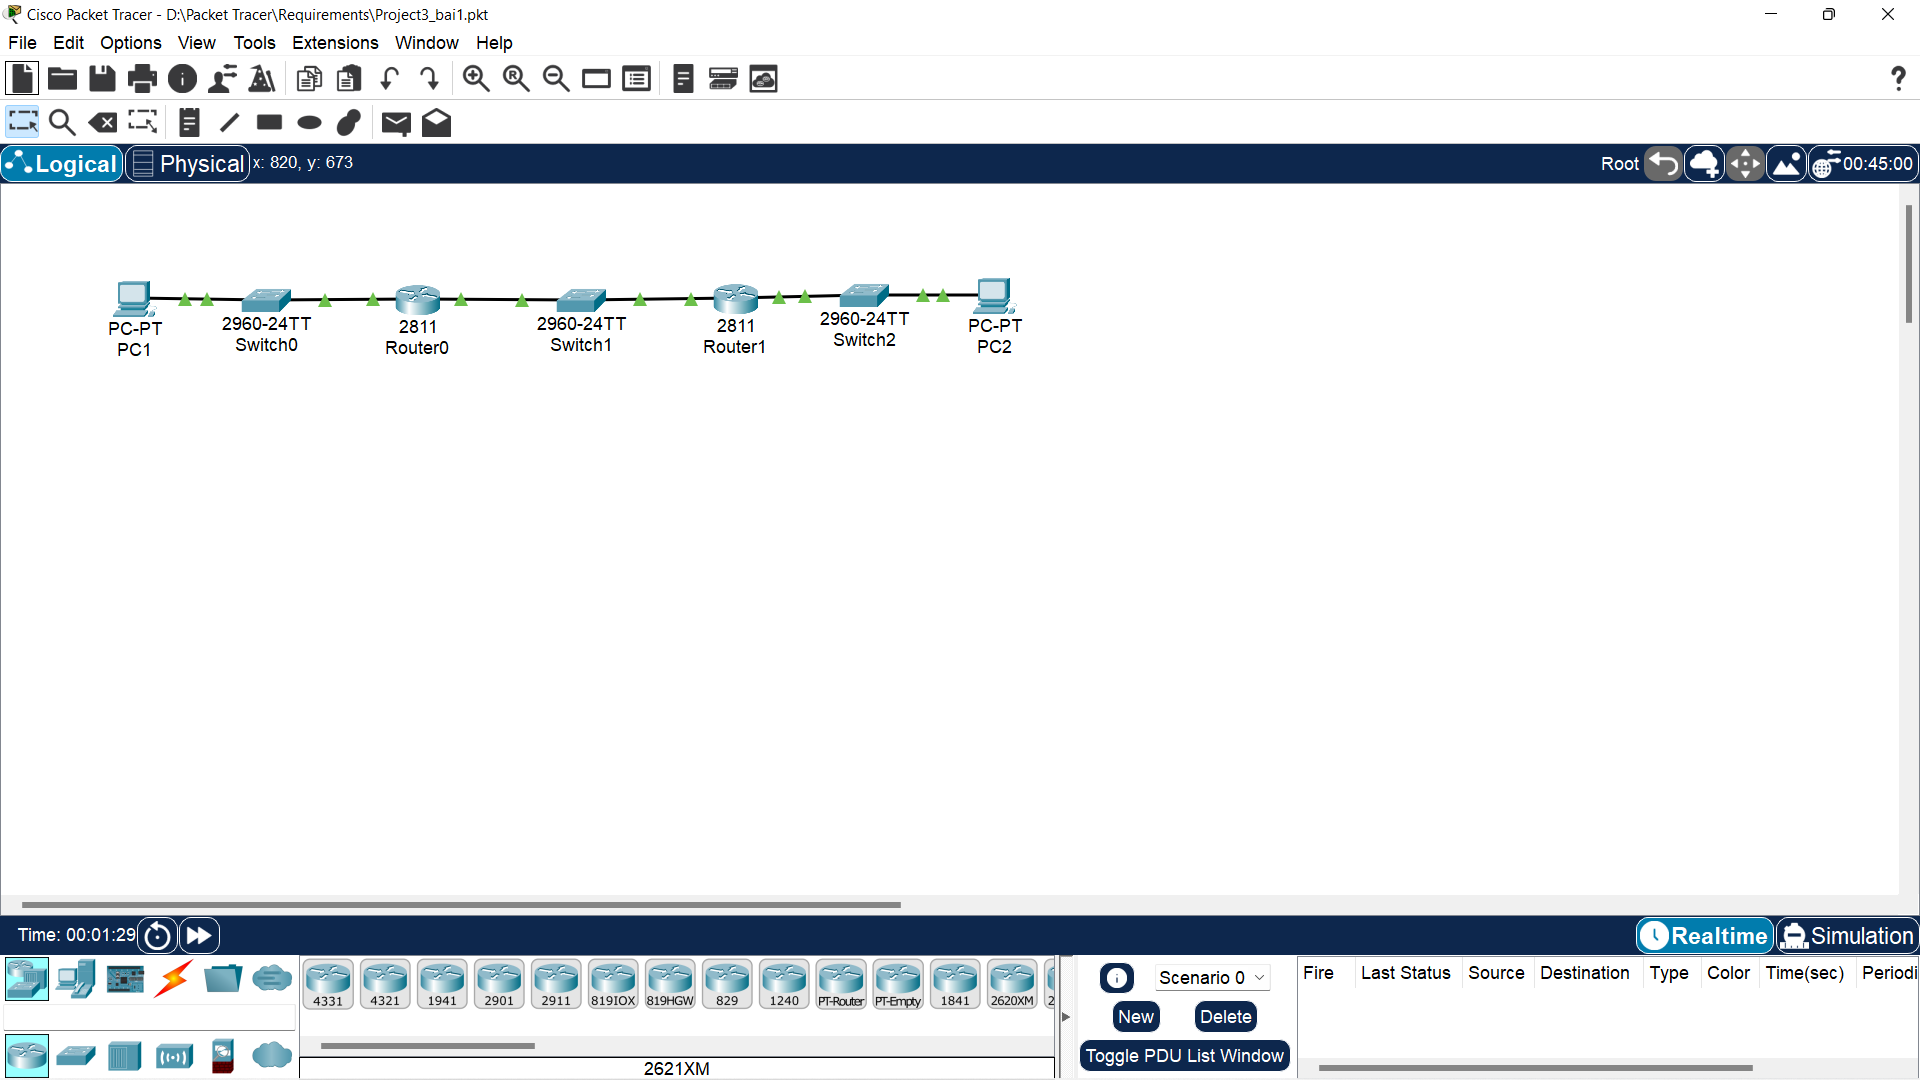
\includegraphics[scale=0.5]{../figures/p1/p1-prob}
\end{center}
\caption{Nội dung tập tin Project3{\_}1.pkt ban đầu}
\label{fig1.1}
\end{figure}

\begin{figure}[H]
\begin{center}
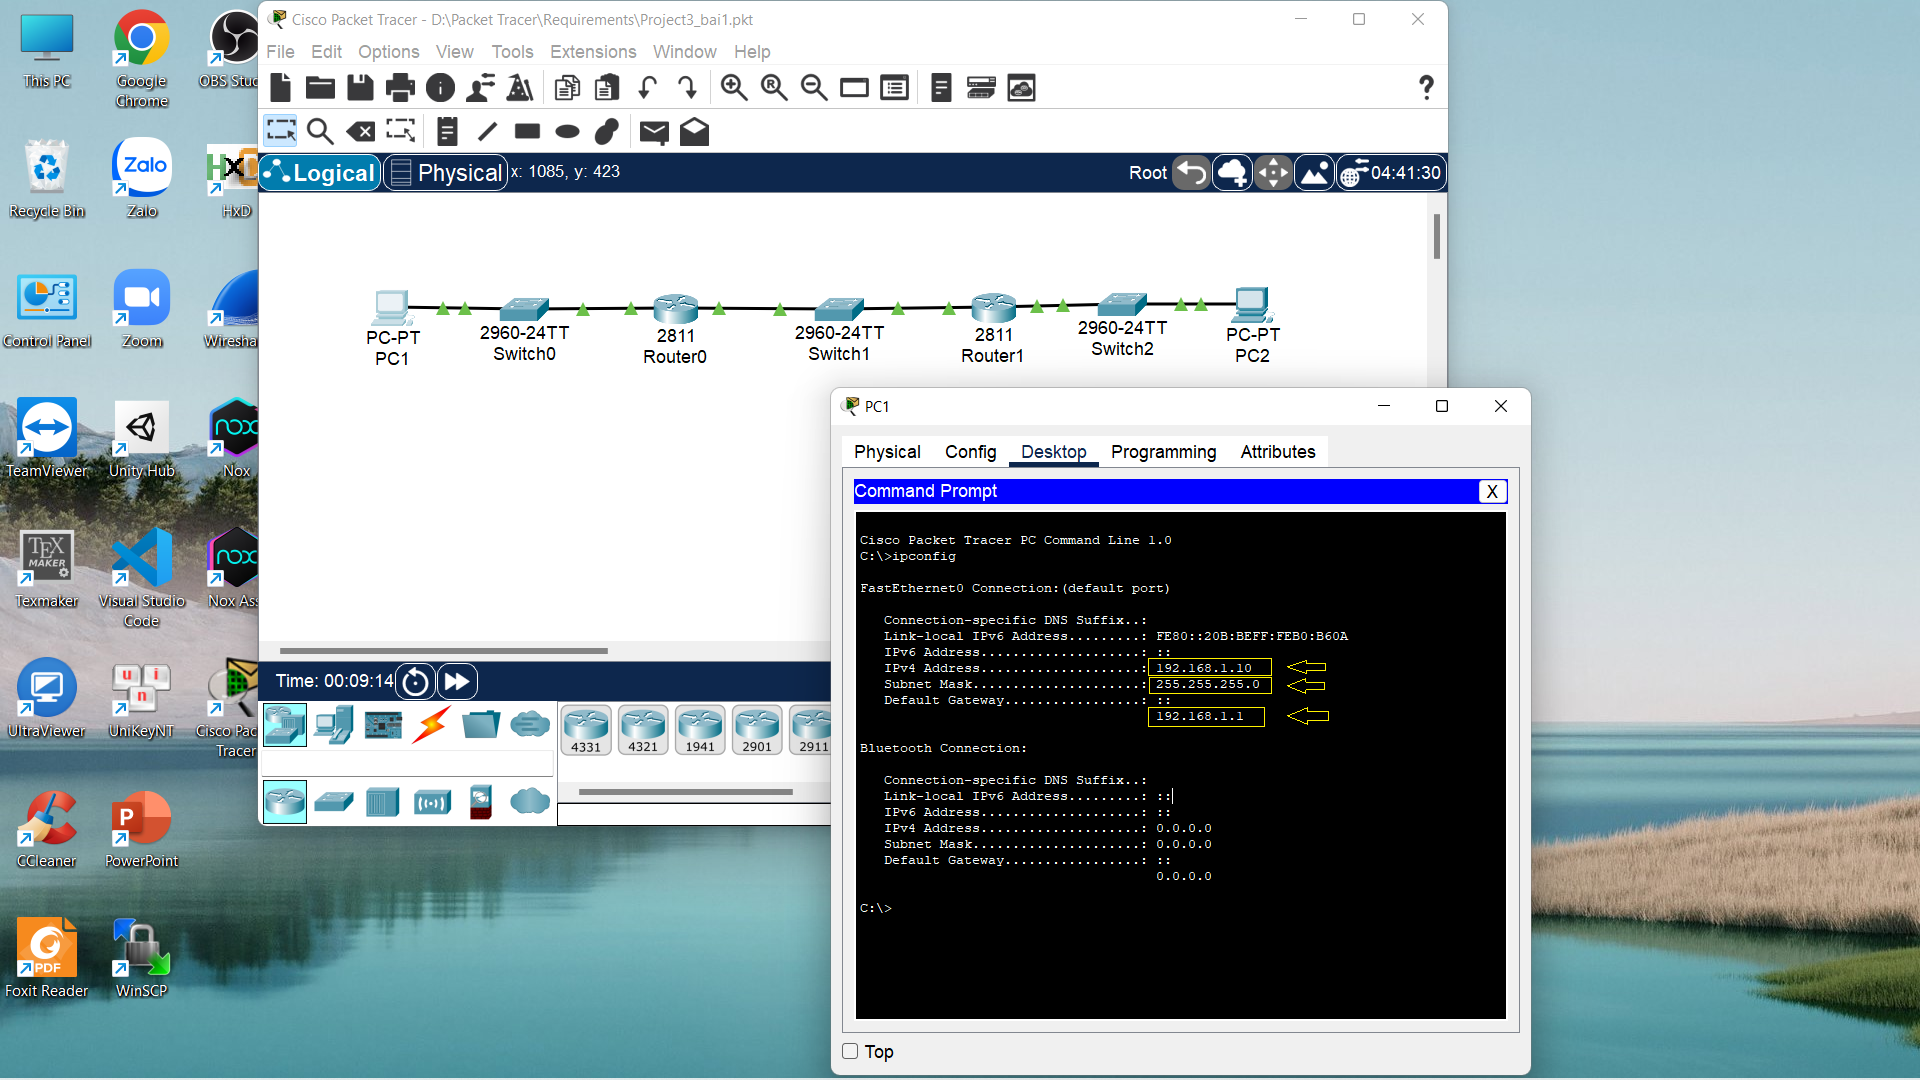
\includegraphics[scale=0.5]{../figures/p1/p1-ipconfig-pc}
\end{center}
\caption{Kiểm tra thông tin IP của PC}
\end{figure}

\begin{figure}[H]
\begin{center}
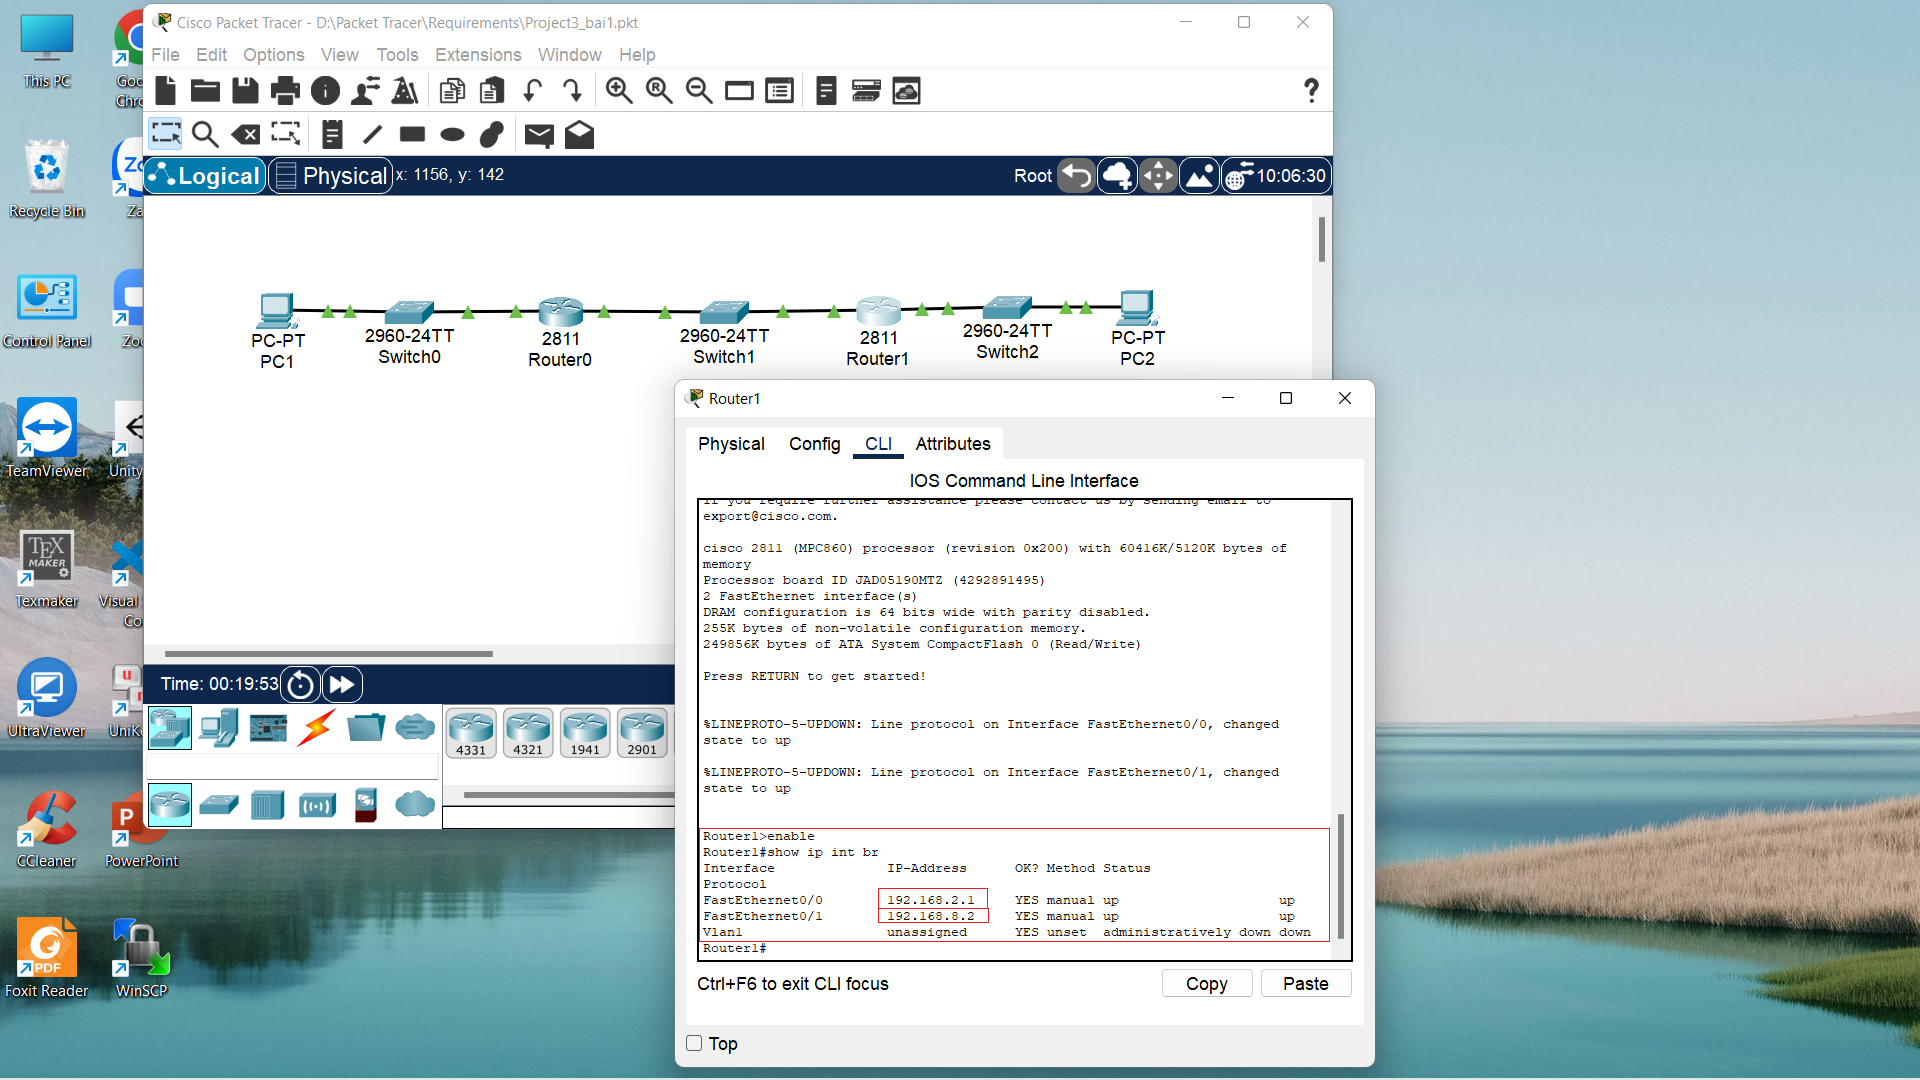
\includegraphics[scale=0.5]{../figures/p1/p1-ipconfig-router}
\end{center}
\caption{Kiểm tra thông tin IP của router}
\end{figure}

\bf \item Ghi chú đầy đủ các thông tin interface, địa chỉ đường mạng, địa chỉ IP lên mô hình mạng:

\rm 
\begin{figure}[H]
\begin{center}
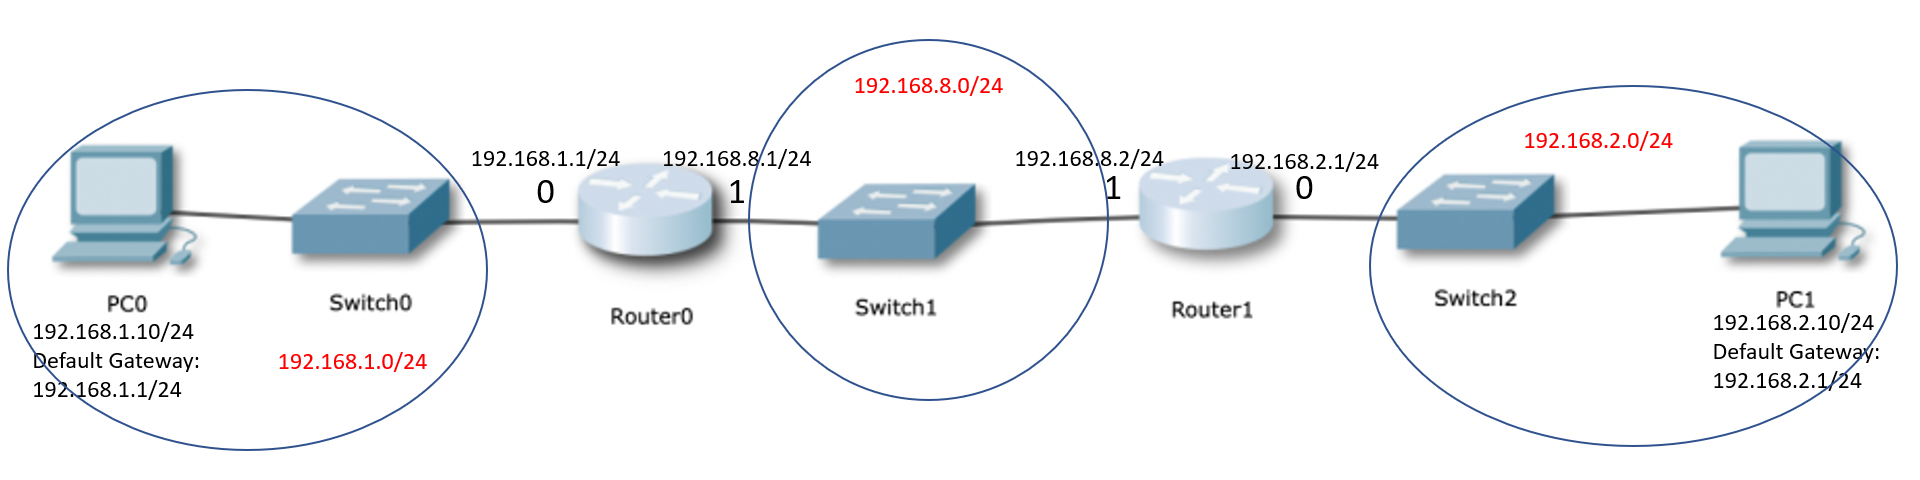
\includegraphics[scale=0.5]{../figures/p1/p1-2}
\end{center}
\caption{Mô hình mạng}
\end{figure}

\bf \item Hãy cho biết các router có được cấu hình gateway hay không? Nếu có hãy viết thông tin gateway của từng router.

\rm Cả 2 router đều chưa được cấu hình gateway.

\begin{figure}[H]
\begin{center}
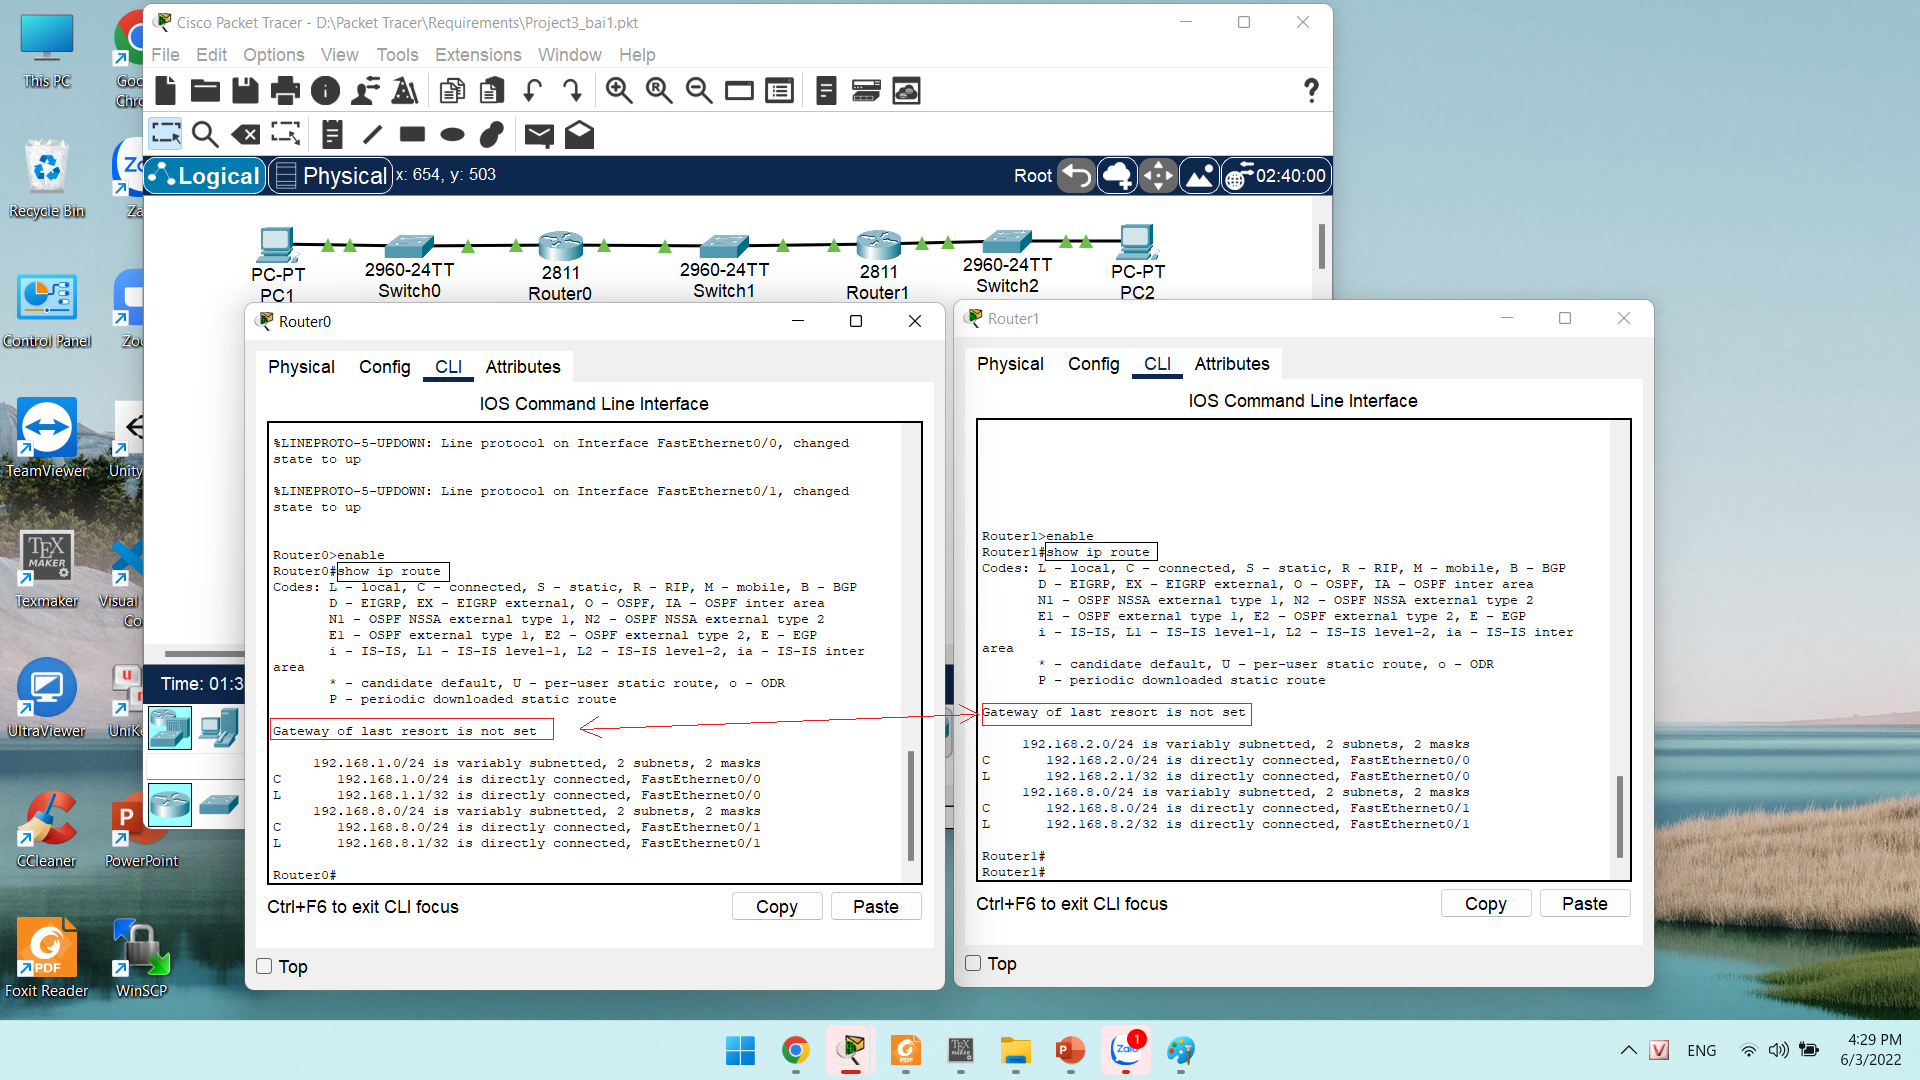
\includegraphics[scale=0.5]{../figures/p1/p1-3}
\end{center}
\caption{Kiểm tra cấu hình gateway}
\end{figure}

\bf \item Kiểm tra kết nối từ PC0 đến PC1, cho biết kết quả như thế nào? (ở lần ping đầu tiên các gói tin ICMP có được gửi thành công hay không). Cho biết đường đi của gói tin ICMP (đi qua các thiết bị, IP nào?)

\rm 

\begin{figure}[H]
\begin{center}
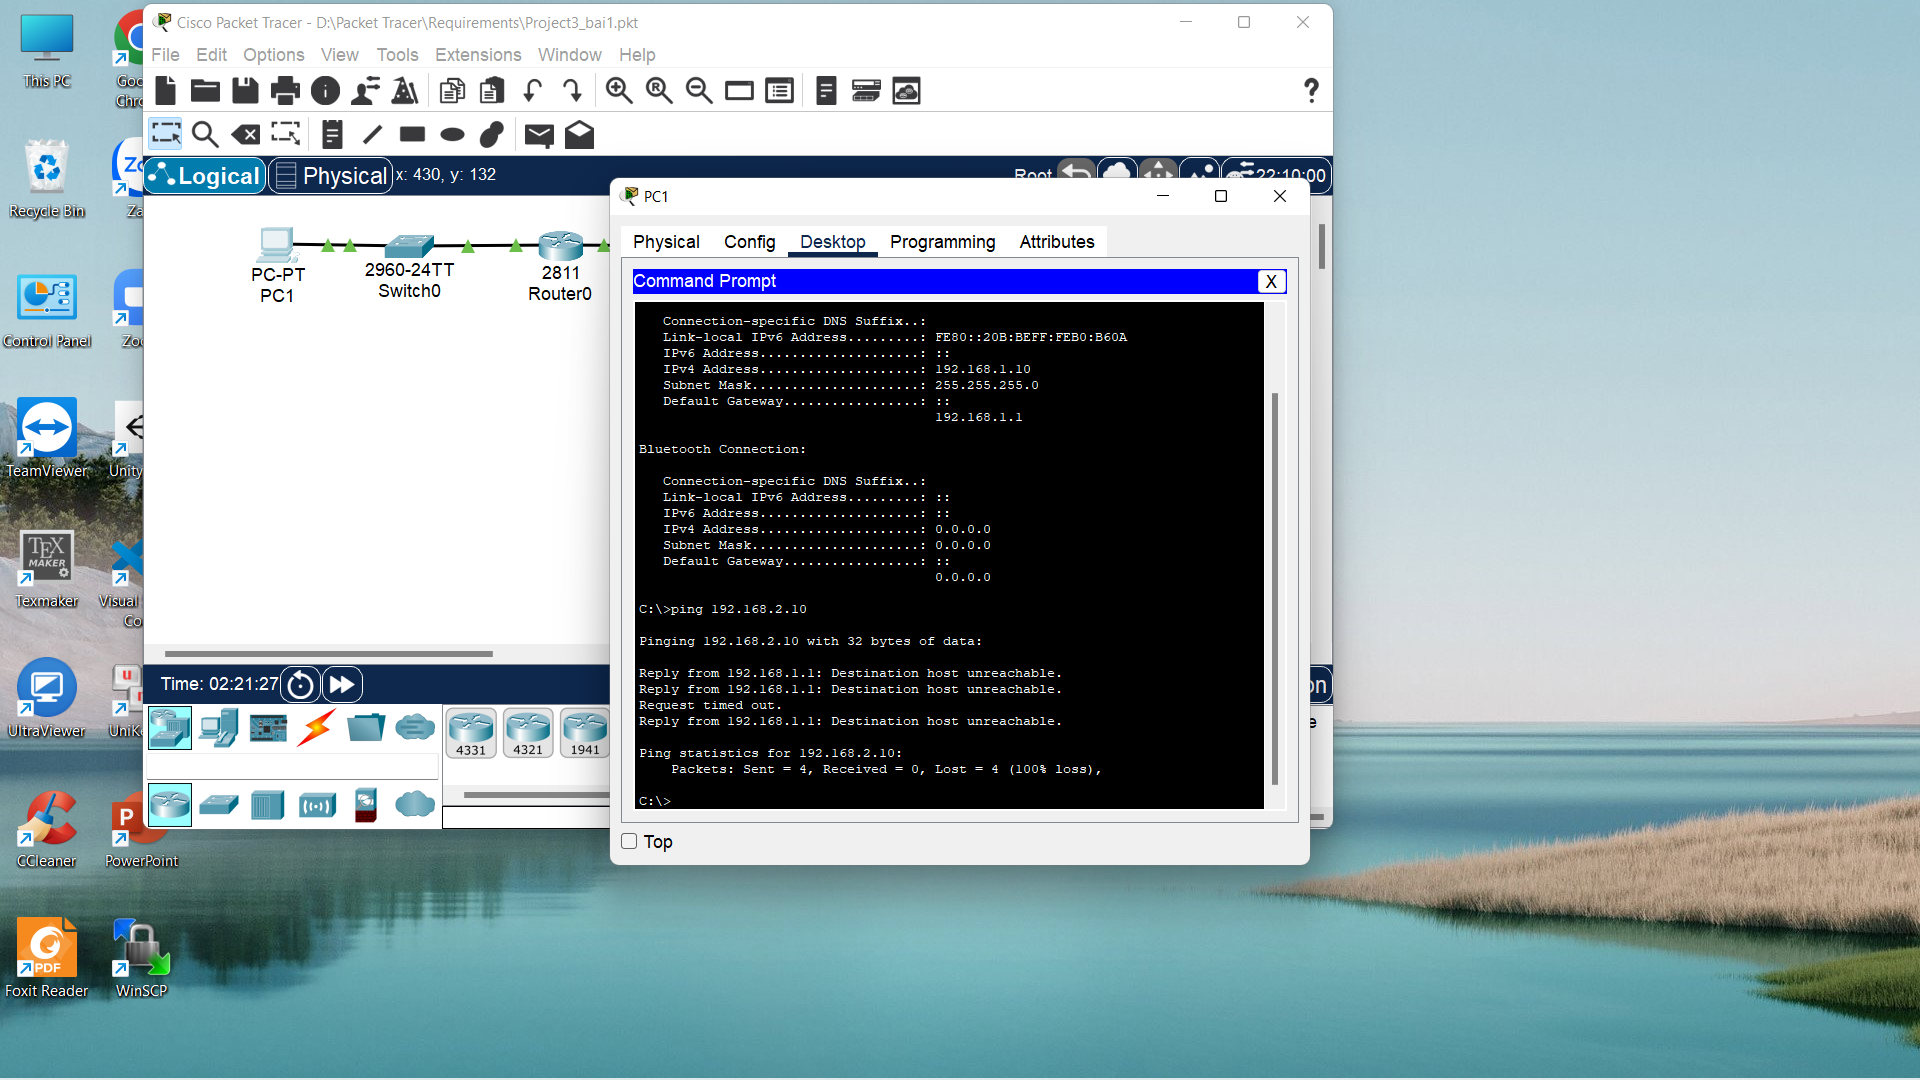
\includegraphics[scale=0.5]{../figures/p1/p1-4}
\end{center}
\caption{Kiểm tra kết nối từ PC0 (\texttt{192.168.1.10}) đến PC1 (\texttt{192.168.2.10})}
\end{figure}

Lúc này cả 2 router chưa cấu hình thông tin định tuyến, do đó máy PC0 trong mạng \texttt{192.168.1.0/24} chưa thể kết nối với máy PC2 trong mạng \texttt{192.168.8.0/24}. Gói tin chỉ đến được router0 cổng 0 (192.168.1.1).

\bf \item Thêm PC2 vào đường mạng \texttt{192.168.8.0/24}. Cấu hình địa chỉ IP, subnetmask, gateway tương ứng cho PC2.

\rm

\begin{figure}[H]
\begin{center}
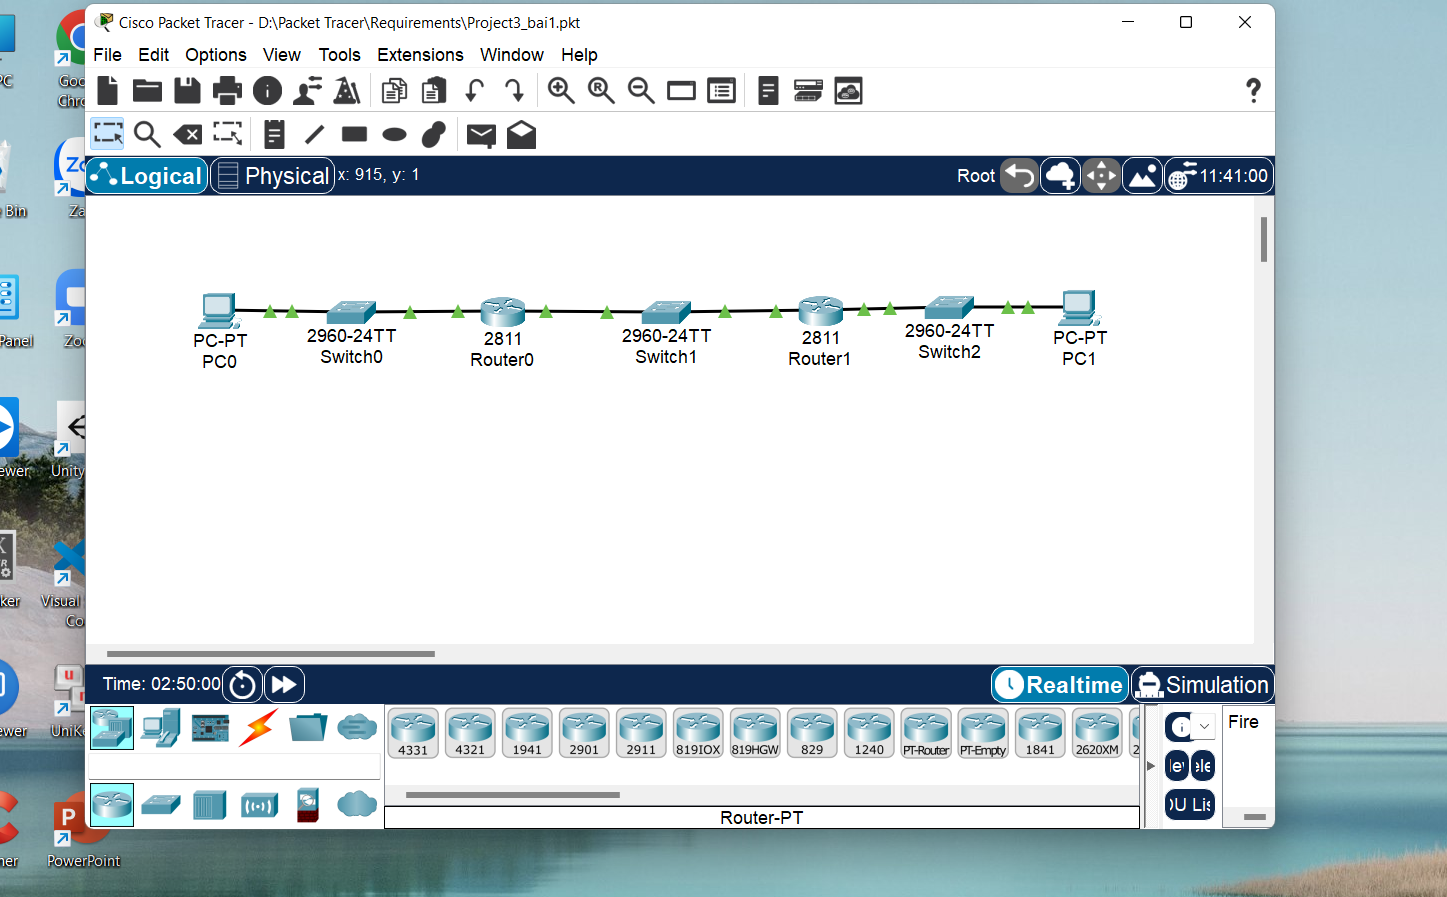
\includegraphics[scale=0.5]{../figures/p1/p1-5a}
\end{center}
\caption{Trước khi thêm PC2}
\end{figure}

\begin{figure}[H]
\begin{center}
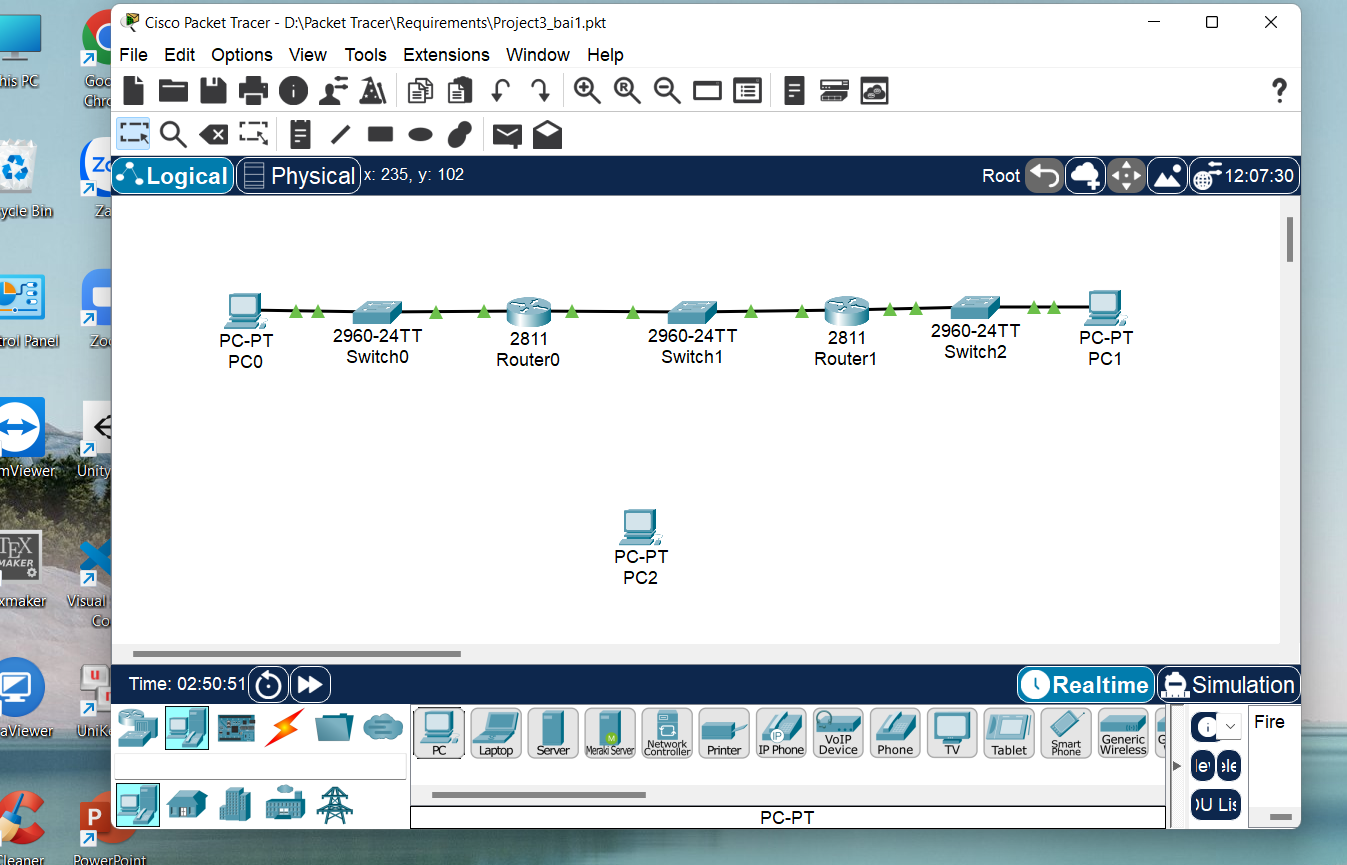
\includegraphics[scale=0.5]{../figures/p1/p1-5b}
\end{center}
\caption{Thêm máy tính mới PC2}
\end{figure}

\begin{figure}[H]
\begin{center}
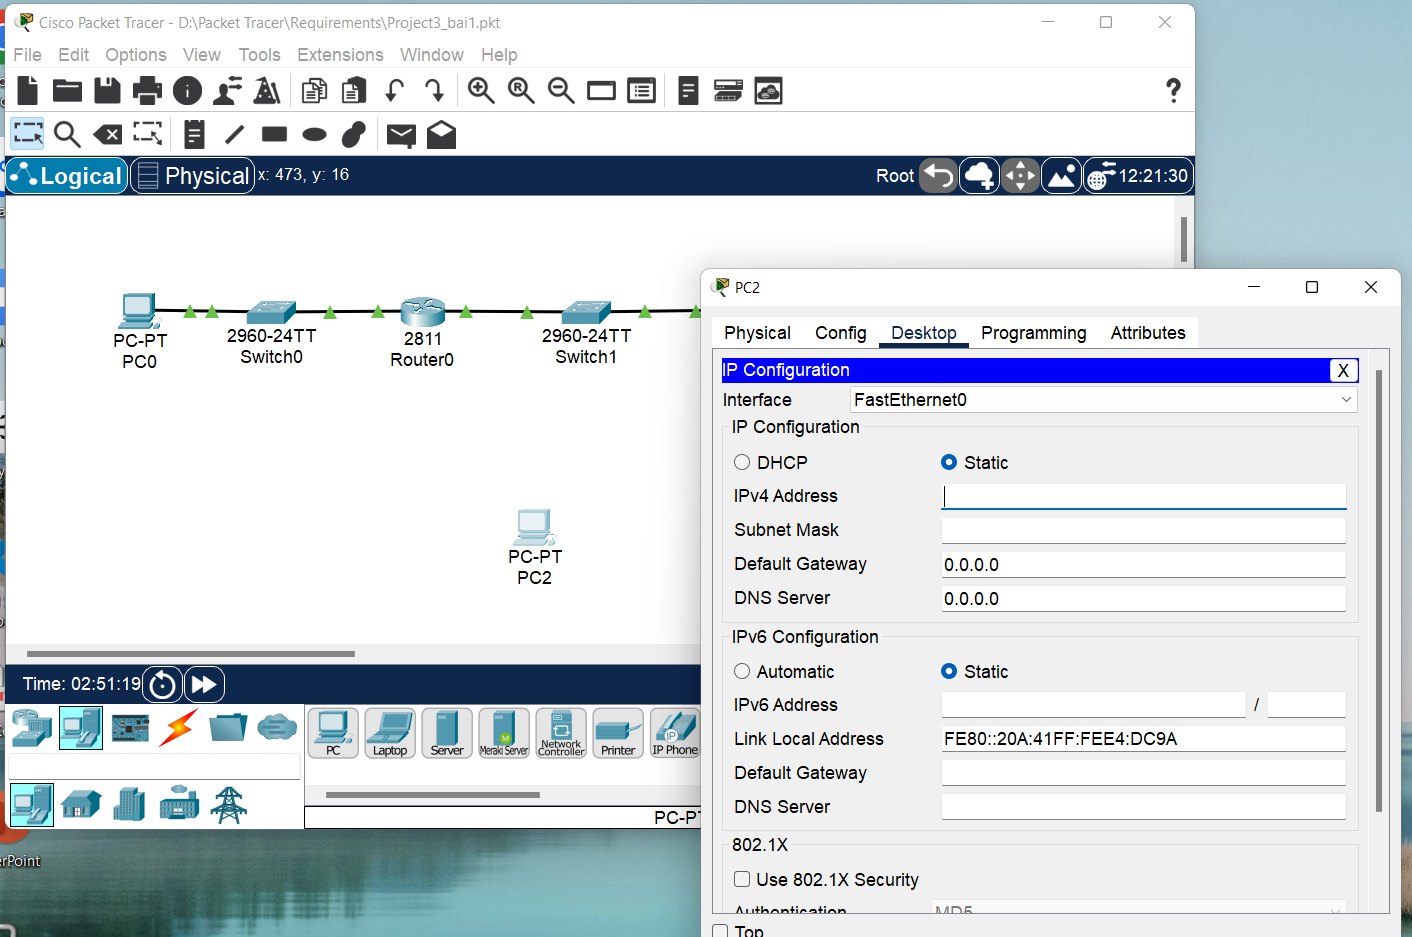
\includegraphics[scale=0.5]{../figures/p1/p1-5c}
\end{center}
\caption{Mở cấu hình máy}
\end{figure}

\begin{figure}[H]
\begin{center}
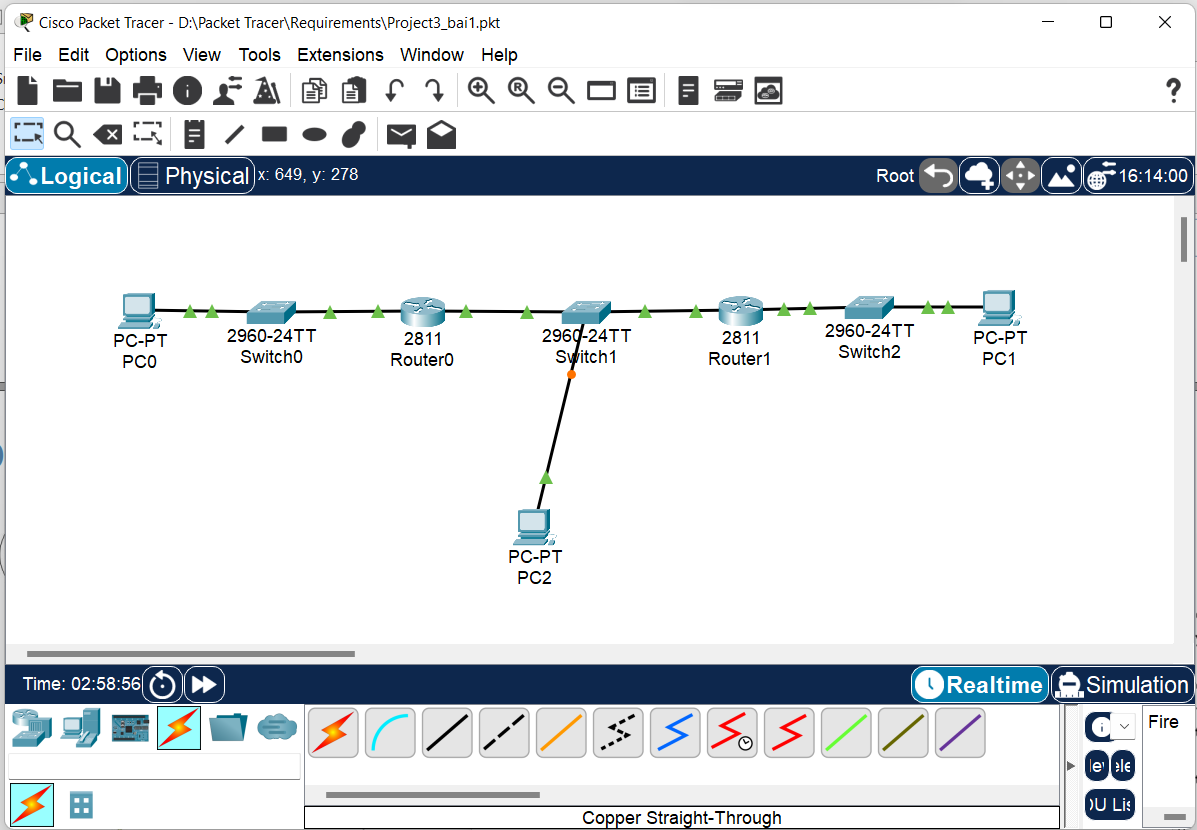
\includegraphics[scale=0.5]{../figures/p1/p1-5d}
\end{center}
\caption{Nối PC2 với Switch1 (Switch1 đang nối 2 router với các cổng \texttt{192.168.8.1} (của Router0), \texttt{192.168.8.2} (của Router1))}
\end{figure}

\begin{figure}[H]
\begin{center}
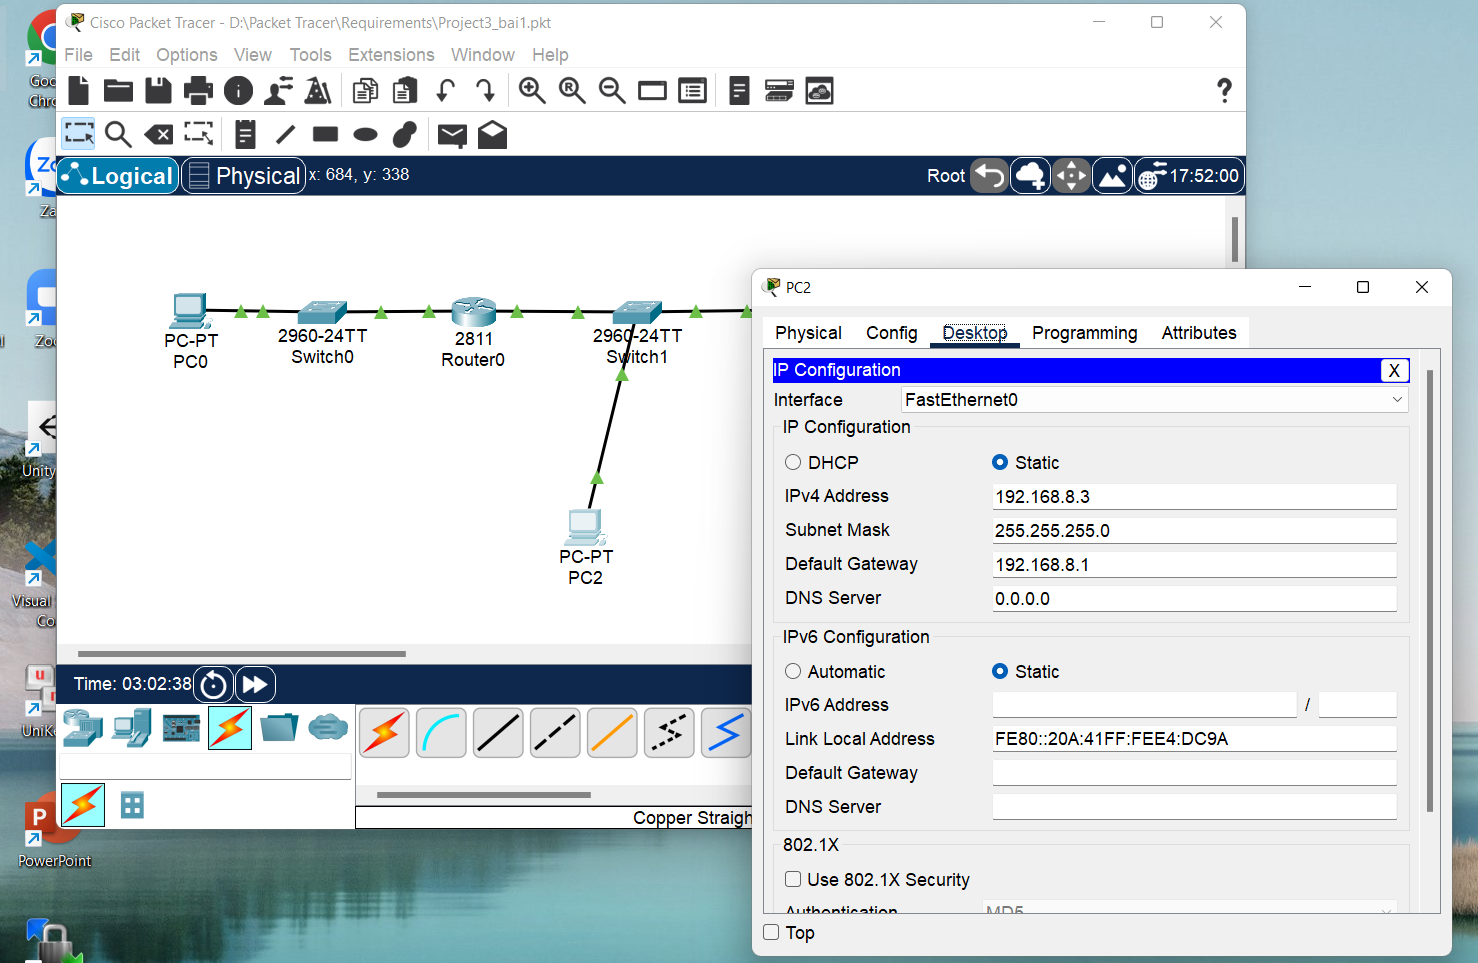
\includegraphics[scale=0.5]{../figures/p1/p1-5e}
\end{center}
\caption{Cấu hình máy PC2, chọn default gateway là \texttt{192.168.8.1}}
\end{figure}


\bf \item Kiểm tra kết nối từ PC0 đến PC2, cho biết kết quả như thế nào? (ở lần ping đầu tiên các gói tin ICMP có được gửi thành công hay không). Cho biết đường đi của gói tin ICMP (đi qua các thiết bị, IP nào?)

\rm 
\begin{figure}[H]
\begin{center}
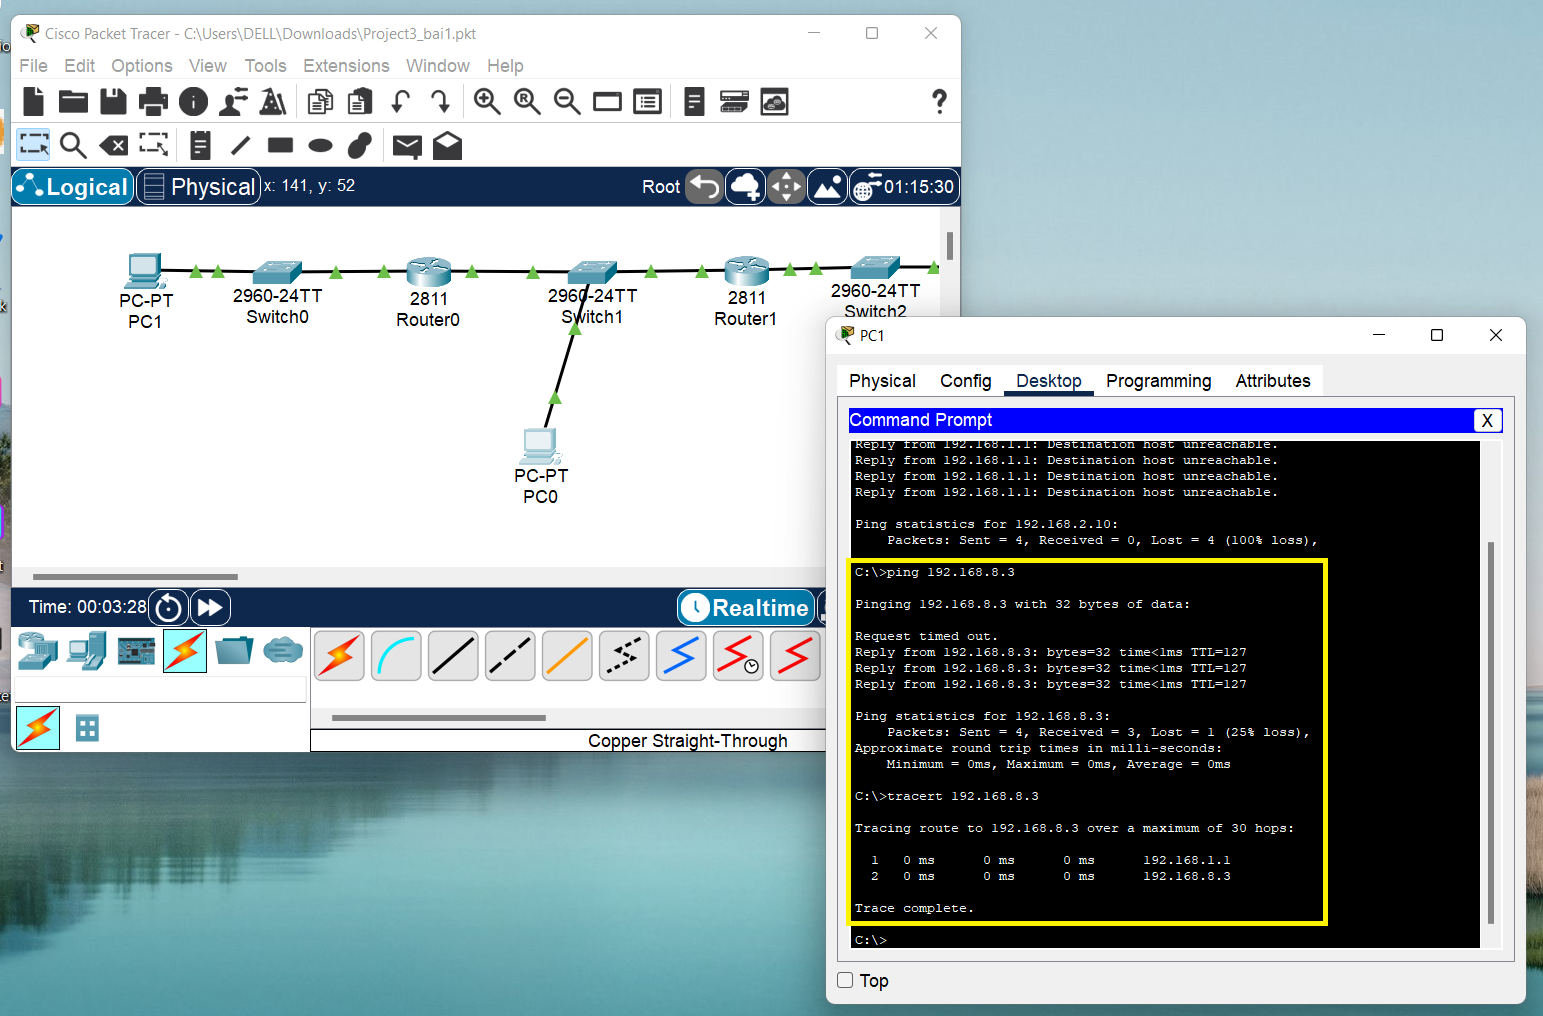
\includegraphics[scale=0.5]{../figures/p1/p1-6}
\end{center}
\caption{Kiểm tra kết nối từ PC0 (\texttt{192.168.1.10}) đến PC2 (\texttt{192.168.8.3})}
\end{figure}

Ở lần \texttt{ping} đầu tiên, có 1 gói tin đầu tiên bị mất, còn lại 3 gói tin kia đều gửi được. Từ lần \texttt{ping} thứ 2, cả 4 gói tin đều gửi được.

Bằng lệnh \texttt{tracert} (hình vẽ) ta thấy được gói tin ICMP đi qua router0, cổng 0: \texttt{192.168.1.1}, sau đó qua cổng 1: \texttt{192.168.8.1} (là default gateway của PC2) đến máy PC2 (\texttt{192.168.8.3}).


\bf \item Thay thế đường default route có trong Router0, Router1 bằng cấu hình định tuyến tĩnh sao cho tất cả các subnet có trong mô hình có thể kết nối lẫn nhau.

\rm Cấu hình static route cho các router:

Click vào router0, mở tab config, vào tab ROUTING/Static, click chuột vào dòng 0.0.0.0/0 via 172.16.1.2 và ấn Remove. Sau đó nhập vào Network 192.168.2.0/24 với Next Hop là 192.168.8.2 và click Add để thêm static route này vào bảng định tuyến. Thực hiện tương tự cho router1.

\begin{figure}[H]
\begin{center}
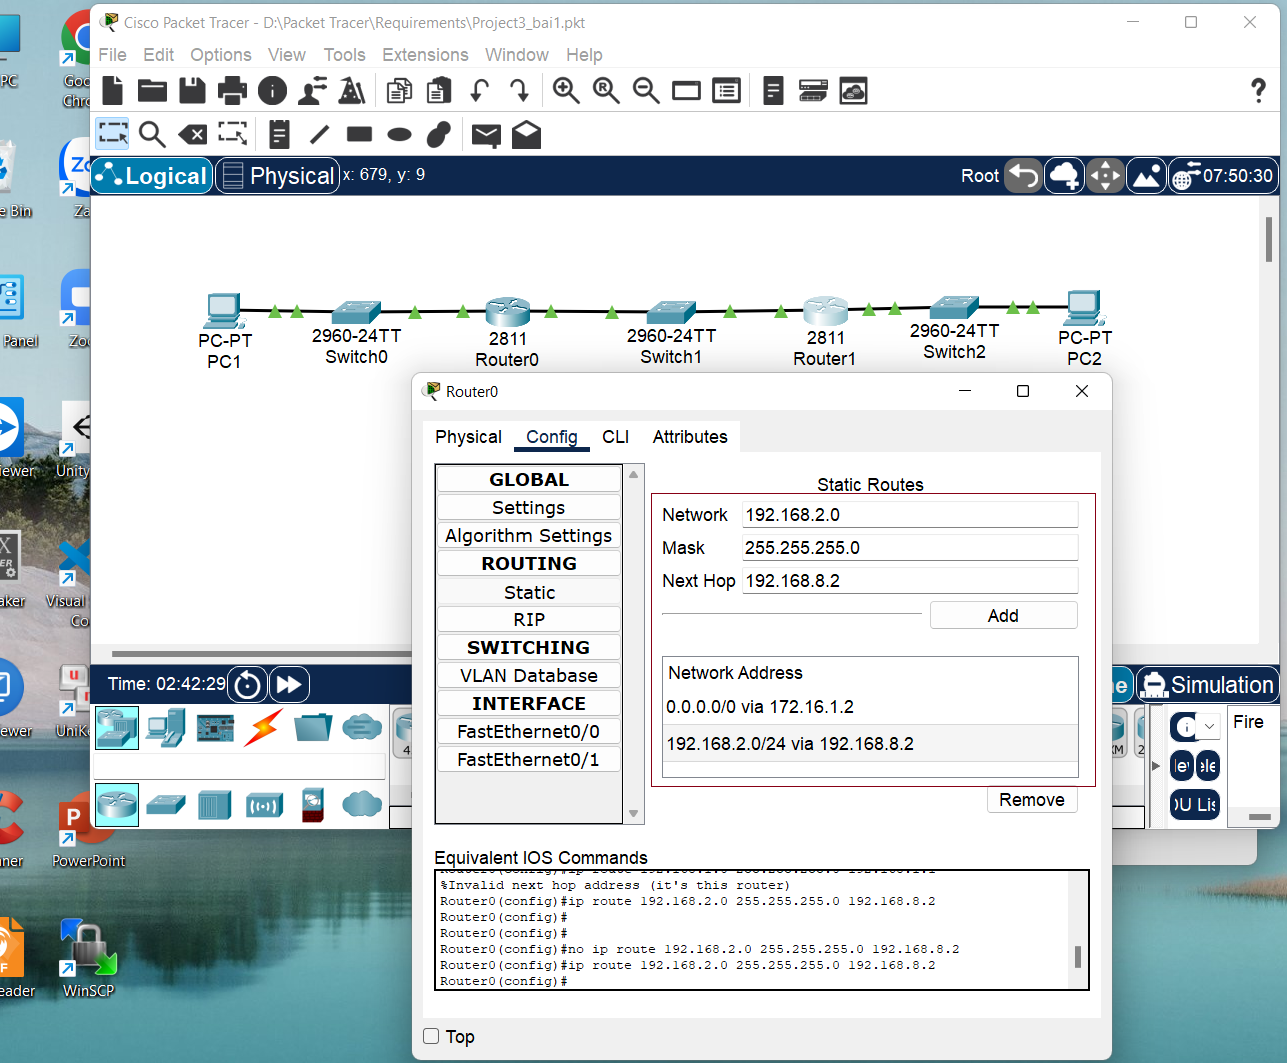
\includegraphics[scale=0.5]{../figures/p1/p1-4a}
\end{center}
\caption{Cấu hình bảng định tuyến cho router0}
\end{figure}

\begin{figure}[H]
\begin{center}
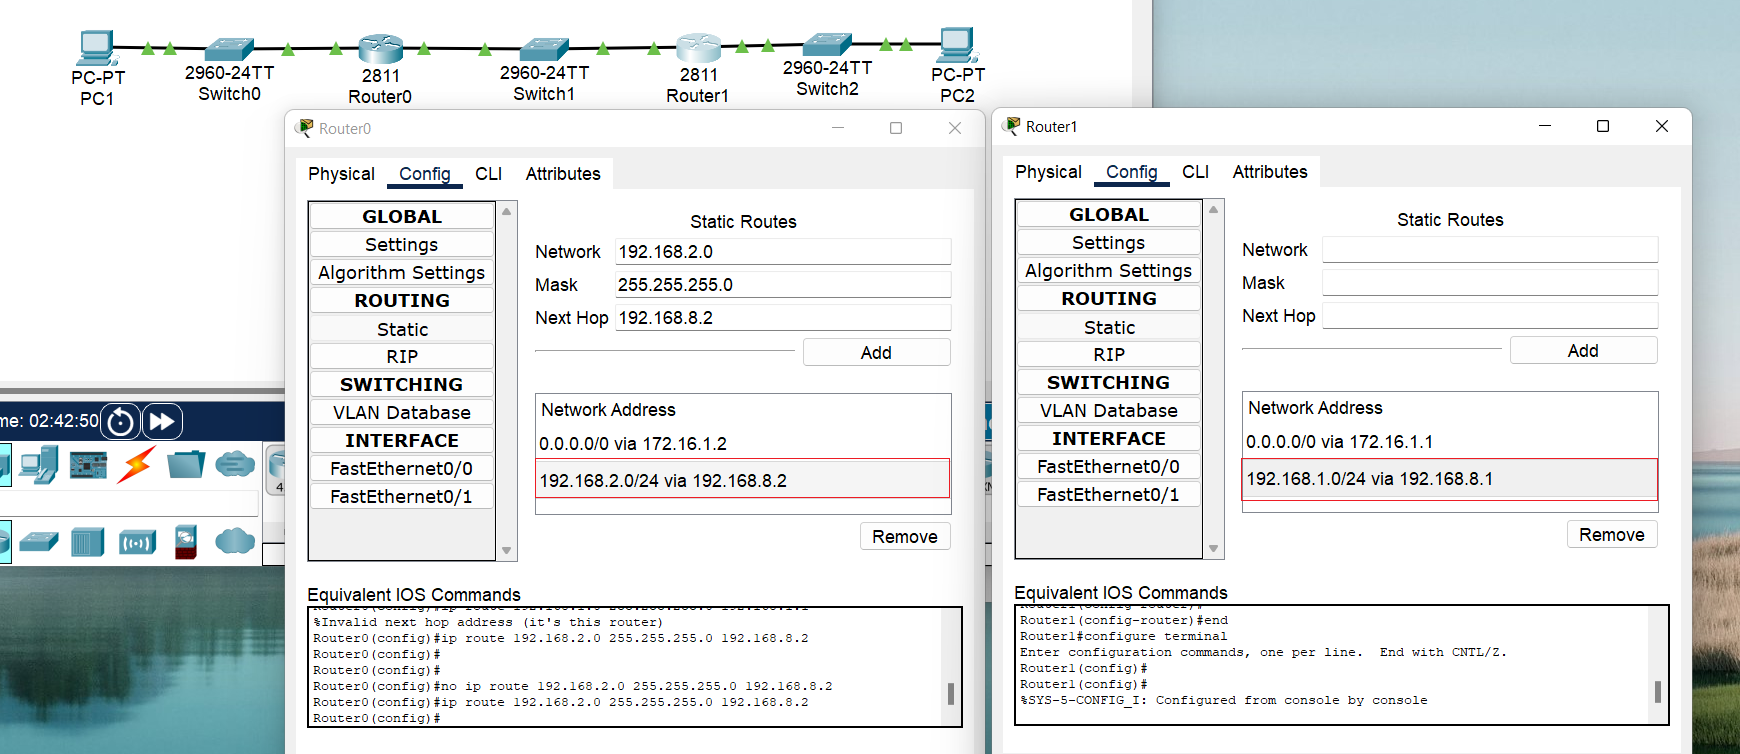
\includegraphics[scale=0.5]{../figures/p1/p1-4b}
\end{center}
\caption{Cấu hình bảng định tuyến cho các router}
\end{figure}

\bf \item Kiểm tra kết nối tất cả các subnet trong mô hình.

\rm Sau khi cấu hình bảng định tuyến cho các router, kết nối được thiết lập, lệnh \texttt{ping} thực hiện được.

\begin{figure}[H]
\begin{center}
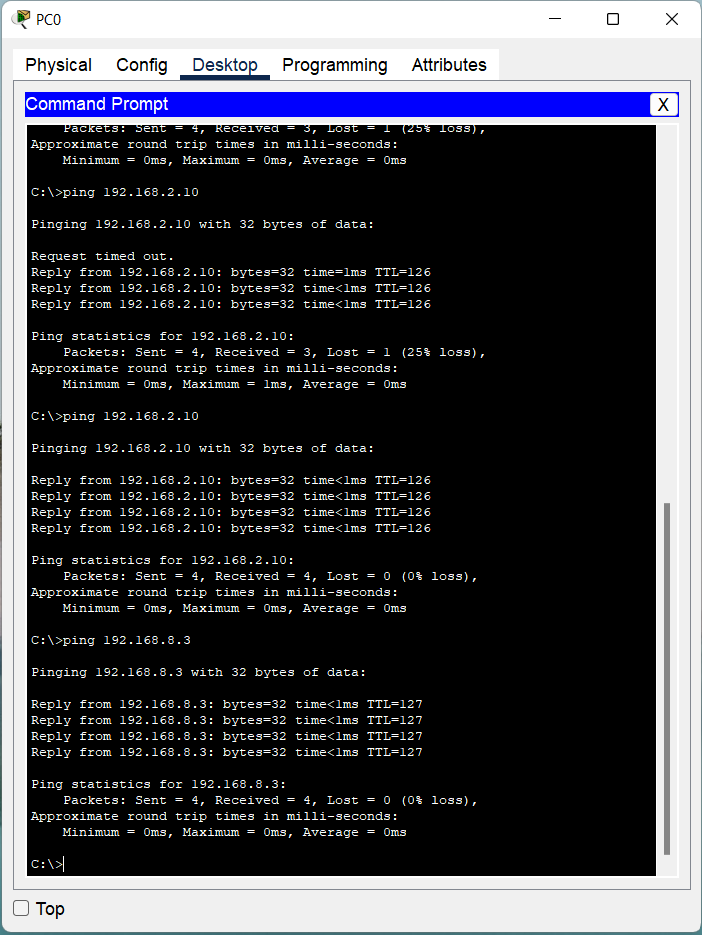
\includegraphics[scale=1]{../figures/p1/p1-70}
\end{center}
\caption{Lệnh \texttt{ping} từ PC0 (\texttt{192.168.1.10}) đến PC1 (\texttt{192.168.2.10}) và PC2 (\texttt{192.168.8.3}) sau khi cấu hình bảng định tuyến tĩnh}
\end{figure}

Lệnh \texttt{ping} từ PC2 sang 2 máy kia:

\begin{figure}[H]
\begin{center}
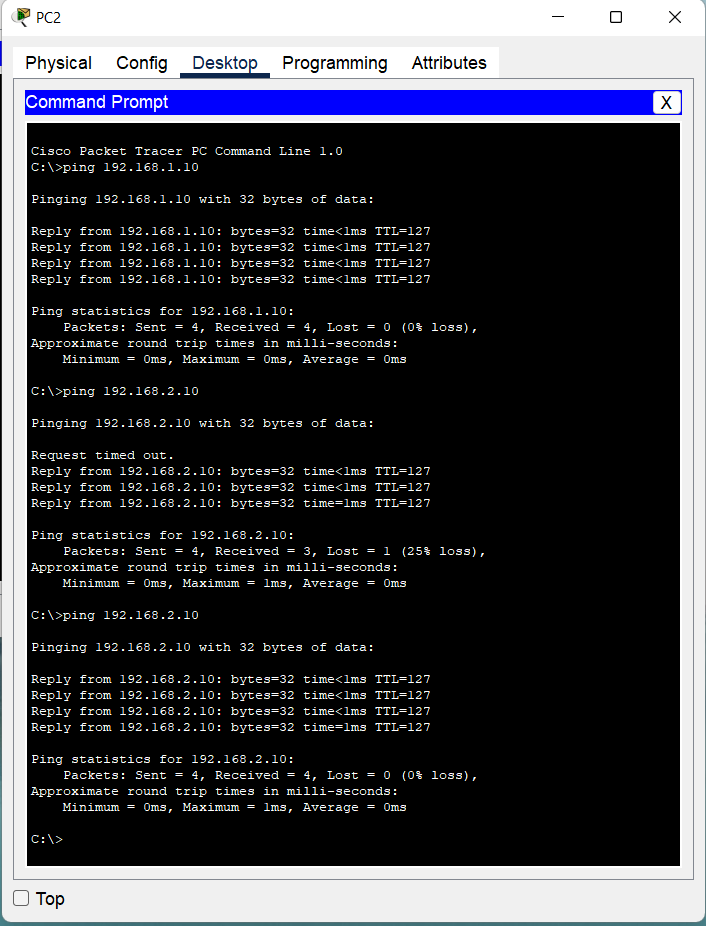
\includegraphics[scale=1]{../figures/p1/p1-72}
\end{center}
\caption{Lệnh \texttt{ping} từ PC2 (\texttt{192.168.8.3}) đến PC0 (\texttt{192.168.1.10}) và PC1 (\texttt{192.168.2.10}) sau khi cấu hình bảng định tuyến tĩnh}
\end{figure}

Lệnh \texttt{ping} từ PC1 sang 2 máy kia:

\begin{figure}[H]
\begin{center}
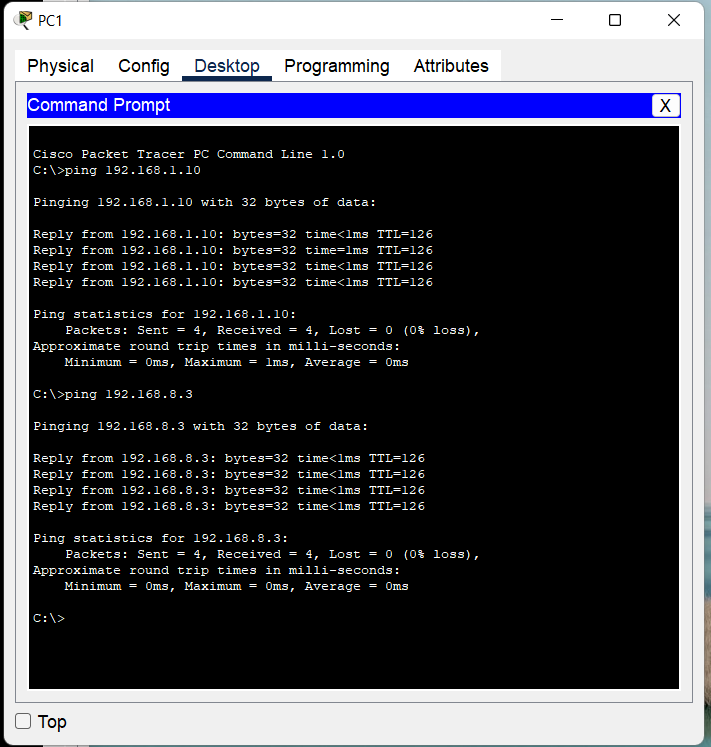
\includegraphics[scale=1]{../figures/p1/p1-71}
\end{center}
\caption{Lệnh \texttt{ping} từ PC1 (\texttt{192.168.2.10}) đến PC0 (\texttt{192.168.1.10}) và PC2 (\texttt{192.168.8.3}) sau khi cấu hình bảng định tuyến tĩnh}
\end{figure}

Kết quả khi kết thúc được lưu trong tập tin \texttt{bai1.pkt}
\end{enumerate}

\newpage
\section{Bài 2:}

Nhóm đóng vai trò là kỹ sư mạng của một công ty, nhóm được giao nhiệm vụ xây dựng hệ thống mạng cho văn phòng mới của công ty.

\bf Mô tả yêu cầu hệ thống:
\begin{enumerate}
\it\item Công ty sử dụng dãy địa chỉ 172.XX.0.0/16 để chia đường mạng cho toàn hệ thống để mỗi phòng/tầng/nhu cầu có đường mạng riêng.

\it\item Tòa nhà của công ty có 4 tầng:
\begin{enumerate}
\sc \item Tầng 1: \rm phòng hành chính (10 users), và một mạng wi-fi cho nhân viên và khách vãng lai (tối đa 20 users)

\sc \item Tầng 2: \rm phòng kỹ thuật (5 users), phòng lãnh đạo (tối đa 5 users)

\sc \item Tầng 3: \rm phòng họp dùng mạng wifi (tối đa 20 users)

\sc \item Tầng 4: \rm phòng server dùng địa chỉ IP tĩnh (tối đa 10 hosts)
\begin{enumerate}
\tt \item Dịch vụ DHCP: \rm triển khai trên 1 server duy nhất/ 1 router để cung cấp dải IP động cho các phòng ban ở tầng 1-2-3

\rm Gợi ý: cấu hình DHCP relay-agent bằng câu lệnh helper-address trên router

\tt \item Dịch vụ DNS phân giải tên miền: \rm mmt-XX.com

\tt \item Dịch vụ WEB \rm để người dùng có thể truy cập trang web công ty từ mạng nội bộ của công ty với tên miền: www.mmt-XX.com. Nội dung trang WEB: hiển thị thông tin MSSV - Họ tên thành viên của nhóm
\end{enumerate}

\sc \item Thiết bị mạng ở các phòng ban có thể kết nối lẫn nhau.
\end{enumerate}
\end{enumerate}

Yêu cầu:
\begin{enumerate}
\bf \item Phân tích hiện trạng và nhu cầu của công ty. Hãy vẽ sơ đồ mạng logic cho văn phòng công ty (có ghi chú tên thiết bị, tên interface/ port, IP, subnet).

\rm 

\bf \item Lập bảng mô tả chi tiết thiết bị gồm: khu vực đặt thiết bị, loại thiết bị, tên thiết bị, version/model, chức năng, tên interface/port, IP

\rm

\bf \item Sử dụng công cụ packet tracer để triển khai mô hình mạng đã thiết kế (chụp hình các bước triển khai cấu hình)

\rm

\bf \item Kiểm tra kết quả hoạt động của mô hình mạng vừa triển khai (dùng các câu lệnh console như ping, nslookup, ipconfig, và trình duyệt web)

\rm Lưu ý:
\begin{enumerate}
\item Chỉ sử dụng phương thức cấu hình định tuyến tĩnh

\item Chỉ sử dụng số lượng PC vừa đủ để kiểm tra hoạt động của mô hình, không cần thiết vẽ đầy đủ số host cho mỗi đường mạng trong mô hình

\item XX là 2 chữ số cuối của MSSV. Nếu làm nhóm 3 người, thì chọn MSSV của một trong 3 bạn.
\end{enumerate}

\end{enumerate}

Trả lời:

\begin{enumerate}
\bf \item Phân tích hiện trạng và nhu cầu của công ty. Hãy vẽ sơ đồ mạng logic cho văn phòng công ty (có ghi chú tên thiết bị, tên interface/ port, IP, subnet).

\rm Hiện trạng và nhu cầu của công ty: Công ty đã có dãy địa chỉ \tt \textcolor{red}{172.72.0.0/16} \rm cần chia cho toàn hệ thống:

\begin{enumerate}
\item Tầng 1: 

\(\bullet\) 1 đường mạng cho phòng hành chính - 10 users

\(\bullet\) 1 đường mạng wi-fi cho nhân viên + khách vãng lai - tối đa 20 users

\item Tầng 2:

\(\bullet\) 1 đường mạng cho phòng kỹ thuật - 5 users

\(\bullet\) 1 đường mạng cho phòng lãnh đạo - tối đa 5 users

\item Tầng 3:

\(\bullet\) 1 đường mạng wi-fi cho phòng họp - tối đa 20 users

\item Tầng 4:

\(\bullet\) 1 đường mạng cho tối đa 10 servers.

\end{enumerate}

Ta thực hiện chia subnet như sau:

Có tổng cộng 6 subnets, trong đó subnet cần nhiều hosts/users nhất là 20 \(\Rightarrow\) cần giữ lại \(m\) bit host sao cho \(2^m-2\ge 20\Rightarrow m\ge 5\), do đó ta được mượn tối đa \(32-16-5 = 11\) bit net. Trong đó ta chỉ cần 6 subnets do đó ta chỉ cần mượn 3 bit (ở byte 3), chia được thành 8 địa chỉ đường mạng con (subnet), mỗi subnet này cho phép số địa chỉ host hợp lệ là \(2^{32-16-3}-2 = 8190 > 20\).

\begin{tabular}{|c|c|c|c|c|}
\hline
STT & Đ/c đường mạng & Subnet mask & Đ/c broadcast & Dải đ/c host hợp lệ\\
\hline
1 & 172.72.0.0 & 255.255.224.0 & 172.72.31.255 & 172.72.0.1 - 172.72.31.254\\
\hline
2 & 172.72.32.0 & 255.255.224.0 & 172.72.63.255 & 172.72.32.1 - 172.72.63.254\\
\hline
3 & 172.72.64.0 & 255.255.224.0 & 172.72.95.255 & 172.72.64.1 - 172.72.95.254\\
\hline
4 & 172.72.96.0 & 255.255.224.0 & 172.72.127.255 & 172.72.96.1 - 172.72.127.254\\
\hline
5 & 172.72.128.0 & 255.255.224.0 & 172.72.159.255 & 172.72.128.1 - 172.72.159.254\\
\hline
6 & 172.72.160.0 & 255.255.224.0 & 172.72.191.255 & 172.72.160.1 - 172.72.191.254\\
\hline
7 & 172.72.192.0 & 255.255.224.0 & 172.72.223.255 & 172.72.192.1 - 172.72.223.254\\
\hline
8 & 172.72.224.0 & 255.255.224.0 & 172.72.255.255 & 172.72.224.1 - 172.72.255.254\\
\hline
\end{tabular}

Ta chia cho từng nhu cầu một đường mạng con (subnet) như sau:

Subnet 1: 172.72.0.0/19 dùng cho phòng hành chính, tầng 1.

Subnet 2: 172.72.32.0/19 dùng cho mạng wi-fi nhân viên và khách vãng lai, tầng 1.

Subnet 3: 172.72.64.0/19 dùng cho phòng kỹ thuật, tầng 2.

Subnet 4: 172.72.96.0/19 dùng cho phòng lãnh đạo, tầng 2.

Subnet 5: 172.72.128.0/19 dùng cho mạng wi-fi phòng họp, tầng 3.

Tầng 4, \(x\le 10\) servers dùng địa chỉ IP tĩnh, ta lấy tương ứng \(x\) địa chỉ trong subnet 6: 172.72.160.0/19, cụ thể là 172.72.160.1 - 172.72.160.\(x\)

Dịch vụ DHCP: triển khai trên server 172.72.160.1

Dịch vụ DNS: triển khai trên server 172.72.160.2

Dịch vụ WEB: triển khai trên server 172.72.160.3


\bf \item Lập bảng mô tả chi tiết thiết bị gồm: khu vực đặt thiết bị, loại thiết bị, tên thiết bị, version/model, chức năng, tên interface/port, IP

\rm

\bf \item Sử dụng công cụ packet tracer để triển khai mô hình mạng đã thiết kế (chụp hình các bước triển khai cấu hình)

\rm

\bf \item Kiểm tra kết quả hoạt động của mô hình mạng vừa triển khai (dùng các câu lệnh console như ping, nslookup, ipconfig, và trình duyệt web)

\rm

\end{enumerate}









\newpage
\section{Bài 3: Traceroute}
Nếu bạn dùng Window thì dùng lệnh \textbf{\textit{tracert}}, nếu bạn dùng Linux/iOS thì bạn dùng lệnh \textbf{\textit{traceroute}}. Lưu ý kết quả bắt gói tin trên Window và Linux/iOS sẽ khác nhau, vì vậy câu trả lời phụ thuộc bạn dùng OS nào.\\
Bật wireshark để bắt gói tin lệnh traceroute từ máy của mình (có thể dùng máy ảo) đến \textbf{\textit{www.fit.hcmus.edu.vn}} (FIT). \\
Bài tập được thực hiện trên máy tính sử dụng hệ điều hành \textbf{Windows 11}.\\
Kết quả bắt gói tin chi tiết được lưu trong tập tin \textbf{bai3.pcapng}.\\

\textbf{1. Chụp hình kết quả bắt gói tin sau khi traceroute hoặc tracert (thấy được những gói tin liên quan).}\\
Kết quả bắt gói tin sau khi tracert như sau.
\begin{figure}[H]
\begin{center}
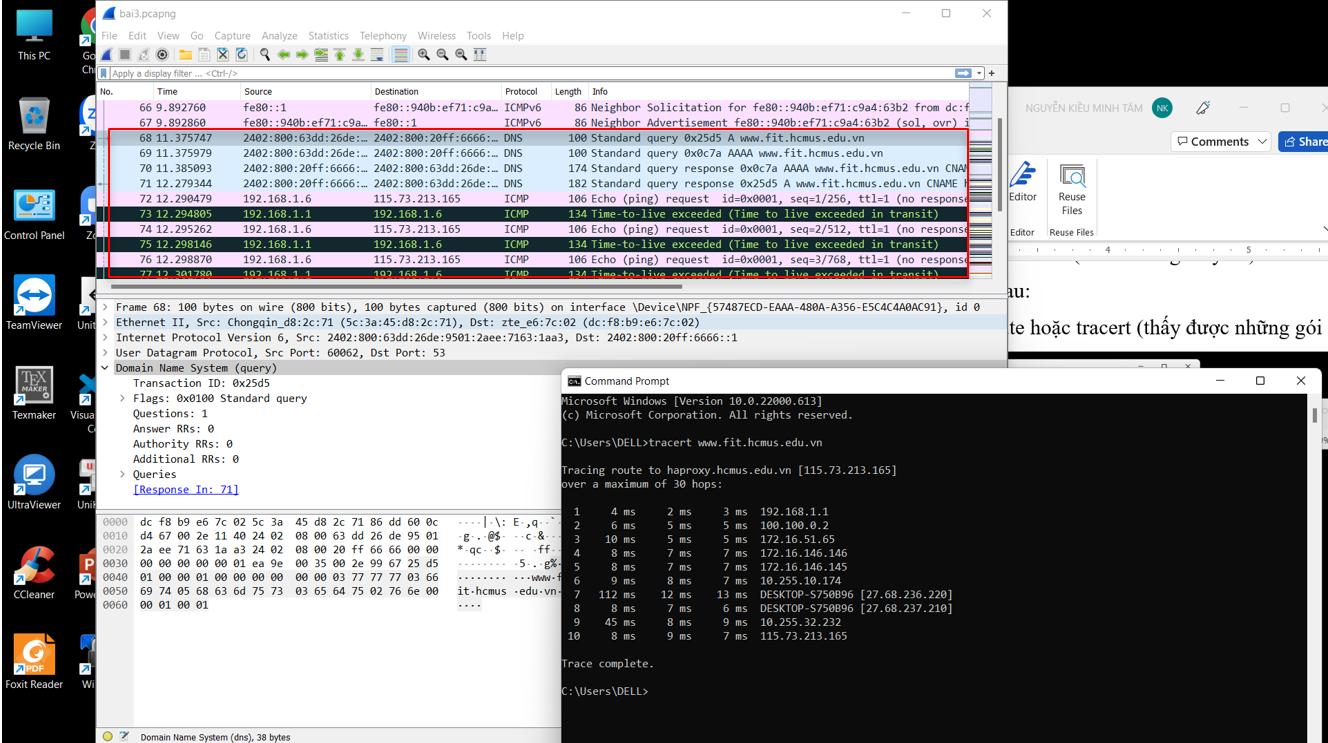
\includegraphics[scale=.8]{../figures/p3/p3_res1}
\end{center}
\caption{Kết quả bắt gói tin sau khi tracert}
\end{figure}
Các gói tin được bắt tính từ lệnh tracert được thể hiện ở phần đóng khung màu đỏ trên hình vẽ. Đó là các gói tin đầu tiên bắt đầu từ khi tracert (gói tin số 68).

\textbf{2. Cho biết traceroute/tracert dùng để làm gì?}\\
Traceroute/tracert dùng để xác định vết đường đi của gói tin giữa hai host: source host và destination host. 
Thông tin này được thể hiện qua các gói tin ICMP (gói tin IP có trường protocol = 1). Và dựa vào thông tin tương ứng trên các trường của thông điệp ICMP, host nguồn xác định được địa chỉ IP của các router trên đường truyền. \supercite{cn, slides}

\textbf{3.	Cho biết địa chỉ IP của máy gửi request.}\\
Địa chỉ IP của máy gửi request là 192.168.1.6.
\begin{figure}[H]
\begin{center}
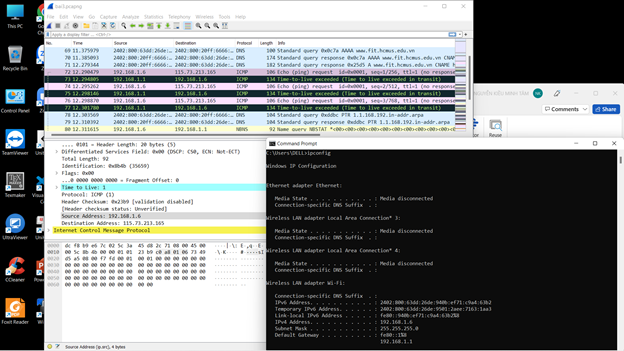
\includegraphics[scale=.8]{../figures/p3/p3_hostip}
\end{center}
\caption{Địa chỉ IP của máy gửi request}
\end{figure}

\textbf{4.	Cho biết cách máy tính xác định được địa chỉ IP của FIT.}\\
Máy tính sẽ gửi gói tin DNS query lên DNS server để “hỏi”, sau đó DNS Server sẽ trả lời qua gói tin DNS response. 
\begin{itemize}
\item Gói tin DNS query được gửi từ destination host là gói tin số 68 (được lưu trong file \textbf{bai3.pcapng}).
\begin{figure}[H]
\begin{center}
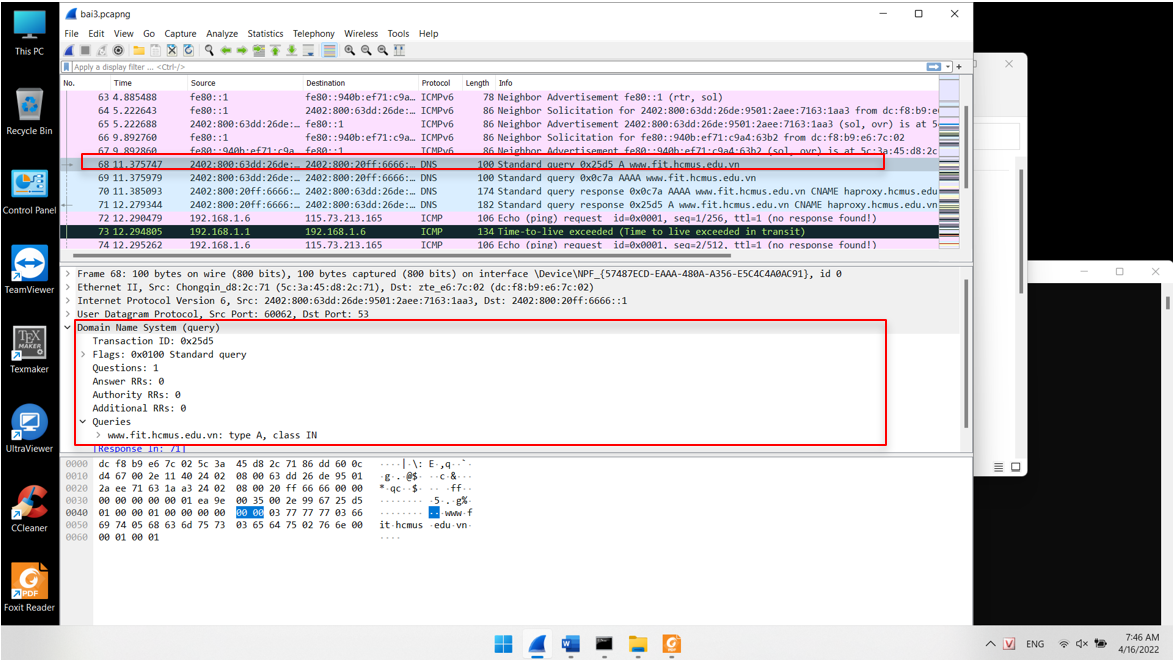
\includegraphics[scale=.8]{../figures/p3/p3_dns1}
\end{center}
\caption{Gói tin DNS query}
\end{figure}
\item Và gói tin trả lời tương ứng là gói tin số 71 (được lưu trong file \textbf{bai3.pcapng}). Hình vẽ cho thấy có FIT có 3 địa chỉ IP 115.73.213.165, 14.161.23.204, 14.241.254.131. Trong lần này traceroute được thực hiện tới địa chỉ IP 115.73.213.165. 
\begin{figure}[H]
\begin{center}
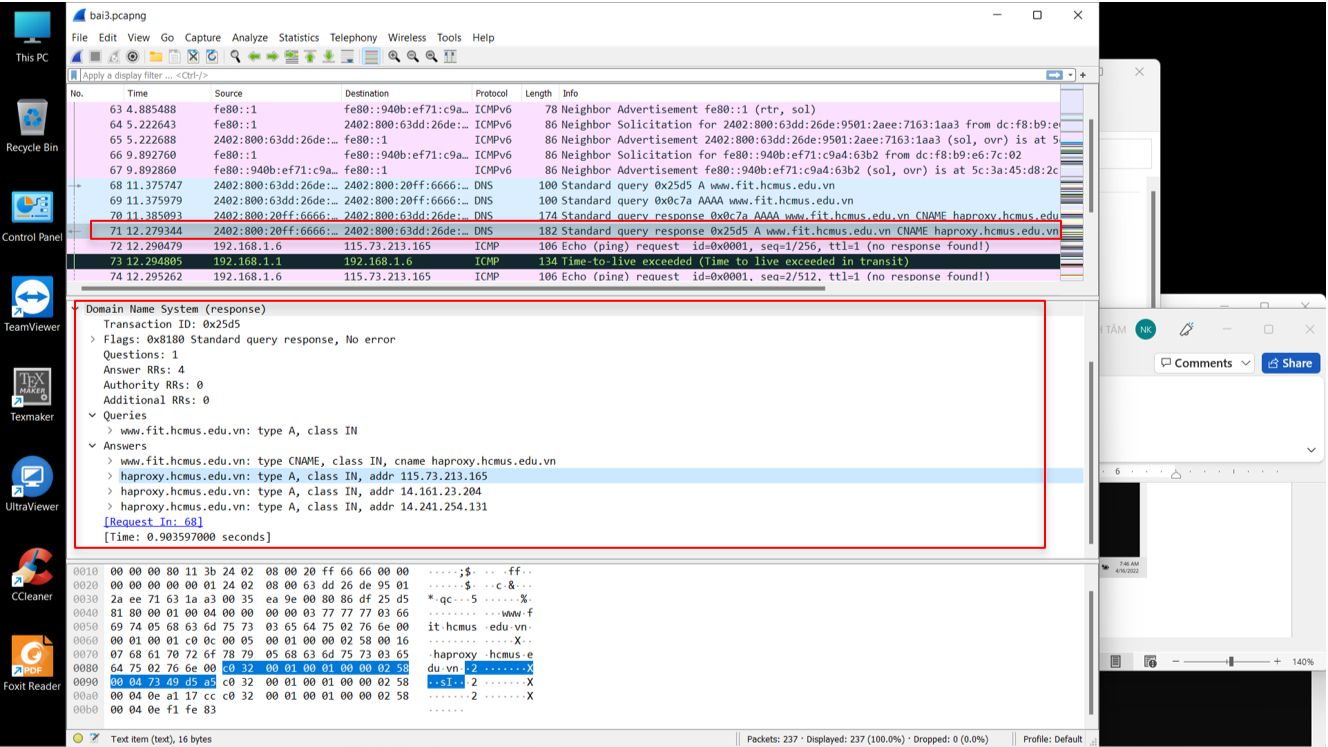
\includegraphics[scale=.8]{../figures/p3/p3_dns2}
\end{center}
\caption{Gói tin DNS query response}
\end{figure}
\end{itemize}

\textbf{5.	Sau khi xác định được IP của www.fit.hcmus.edu.vn, máy sẽ bắt đầu gửi gói tin đến FIT.}\\
\textbf{a.	Protocol được sử dụng của những gói tin sau đó là gì?}\\
Protocol được sử dụng trong những gói tin sau đó là ICMP, bắt đầu từ gói tin số 72 trong file \textbf{bai3.pcapng} (phần đóng khung màu đỏ trong hình \ref{fig351}).

\begin{figure}[H]
\begin{center}
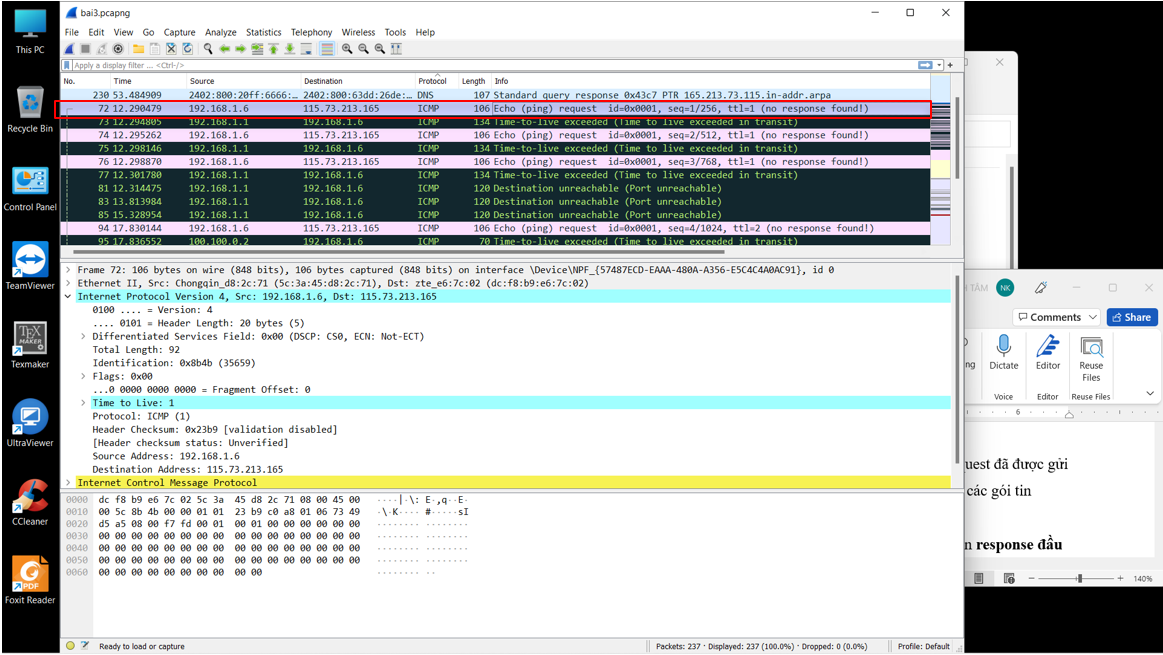
\includegraphics[scale=.8]{../figures/p3/p3_51}
\end{center}
\caption{Protocol được sử dụng}
\label{fig351}
\end{figure}

\textbf{b.	Có bao nhiêu gói tin được gửi đi (request) trước khi nhận được response đầu tiên trả lời cho những request? (Hay nói một cách khác là: lệnh trace* sẽ gửi request message đi, và nhận về response. Vậy có bao nhiêu gói tin request đã gửi đi đến khi nhận được gói tin response đầu tiên?)}\\
Tính từ gói tin request đầu tiên (gói tin số 72) có tổng cộng \textbf{28 gói tin} request đã được gửi trước khi nhận được respone message đầu tiên (gói tin số 224), không kể các gói tin không liên quan khác.

\textbf{c.	Cho biết TTL của gói tin cuối cùng được gửi trước khi nhận được gói tin response đầu tiên trả lời cho những gói tin request?}\\
TTL của gói tin cuối cùng được gửi trước khi nhận được gói tin response đầu tiên trả lời cho những gói tin request là 10 (gói tin 223, phần đóng khung màu vàng trong hình \ref{fig352}).
\begin{figure}[H]
\begin{center}
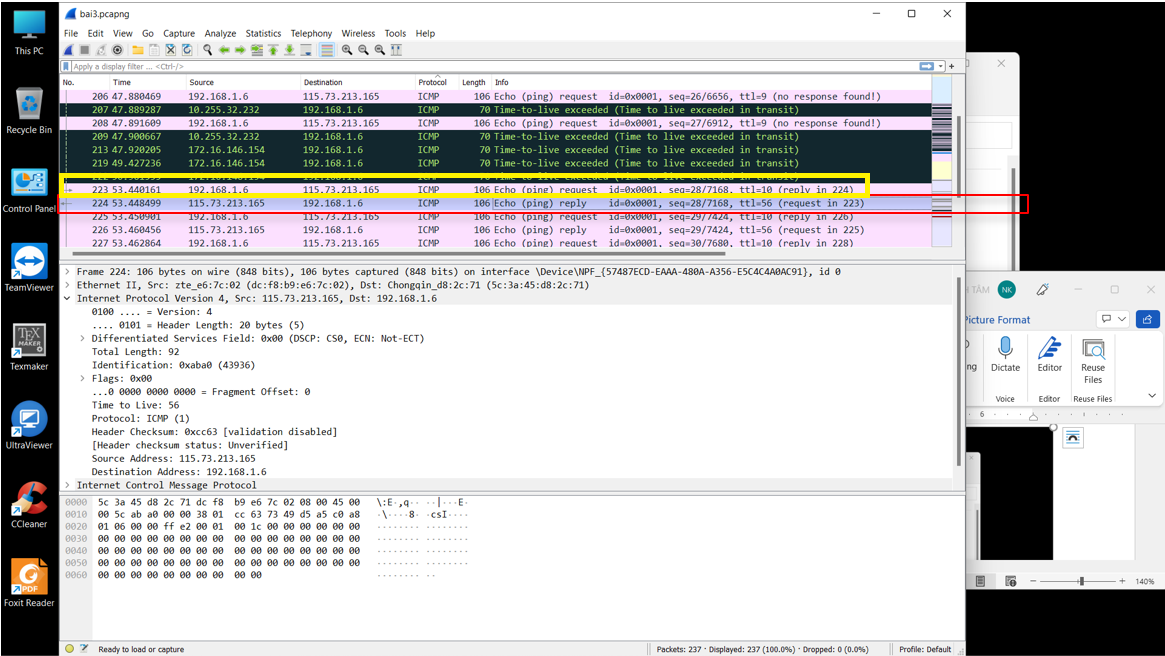
\includegraphics[scale=.8]{../figures/p3/p3_52}
\end{center}
\caption{TTL của gói tin cuối cùng trước khi nhận response}
\label{fig352}
\end{figure}

\textbf{d.	Bạn có thấy thông tin port trong các gói tin gửi đi? Nếu có bạn nhận thấy port nguồn/đích của gói tin có gì đặc biệt? Nếu không thấy thông tin port, hãy giải thích nguyên nhân.}\\
Trong các gói tin gửi đi không tìm thấy thông tin port. Vì nghi thức ICMP hoạt động ở tầng Network, trong khi số hiệu port là “địa chỉ” của ứng dụng, được sử dụng ở tầng Application.

\textbf{e.	Gói tin response đầu tiên là trả lời cho gói tin request thứ mấy? (No.)}\\
Gói tin response đầu tiên (gói tin số 224) trả lời cho gói tin request thứ 28 (gói tin số 223) (phần đóng khung màu đỏ trong hình \ref{fig352}).
\newpage
\section{Bài 4: DHCP}
\newpage
\section{Bài 5: FTP}
Cho tập tin FTP$\_$02.cap, đọc tập tin này bằng Wireshark và trả lời các câu hỏi sau.\\
\textbf{a.	FTP sử dụng giao thức nào UDP hay TCP?}\\
FTP sử dụng giao thức TCP (phần đóng khung màu vàng trong hình \ref{fig5a1}).
\begin{figure}[H]
\begin{center}
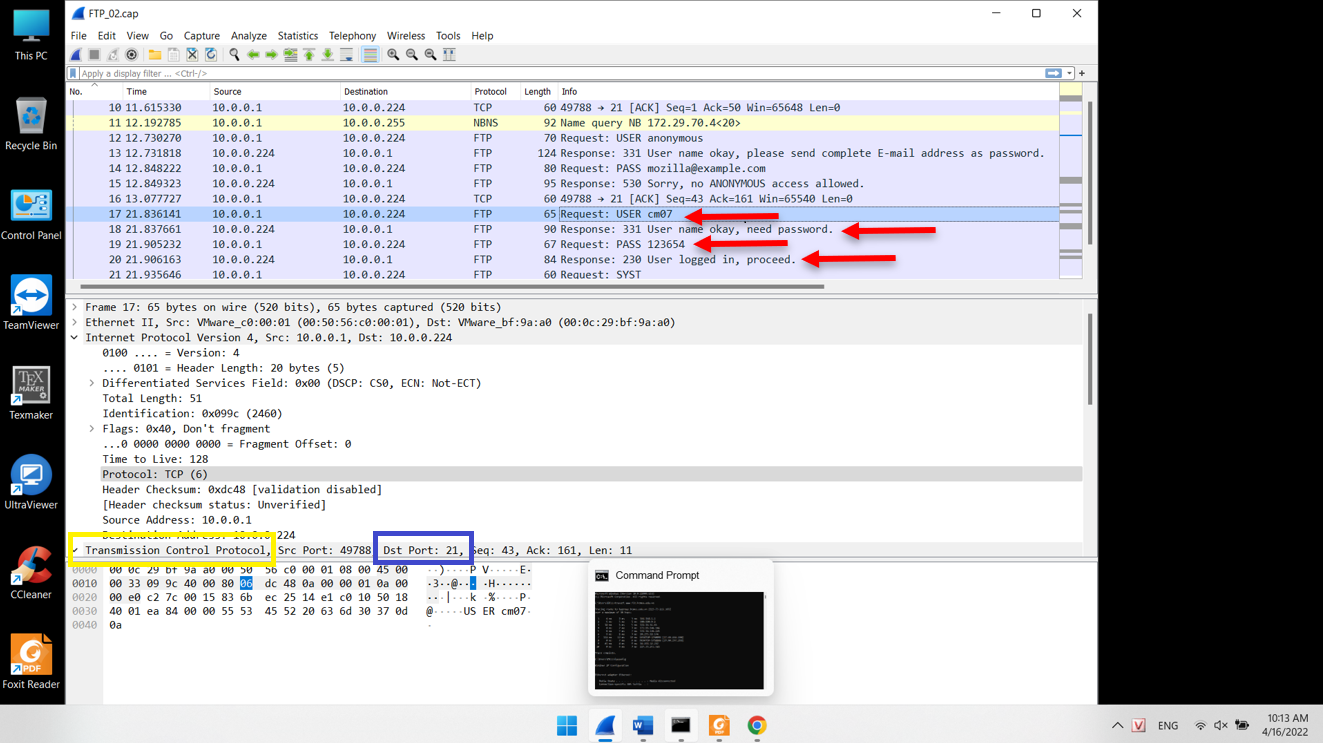
\includegraphics[scale=.8]{../figures/p5/p5_1}
\end{center}
\caption{Giao thức được FTP sử dụng}
\label{fig5a1}
\end{figure}

\textbf{b.	Port mặc định của FTP Server để nhận kết nối là bao nhiêu?}\\
Port mặc định của FTP Server để nhận kết nối là 21 (phần đóng khung màu xanh trong hình \ref{fig5a1}).\\

\textbf{c.	Username và password của người dùng là gì?}\\
Username của người dùng là cm07, password là 123654. Các mũi tên màu đỏ trên hình \ref{fig5a1} thể hiện vị trí thông tin các gói tin tương ứng (các gói tin request, số 17, 19; và các gói tin response tương ứng, số 18, 20). Còn user anonymous ở phía trên không được cho phép kết nối (các gói tin 12 đến 15).

\textbf{d.	Port truyền lệnh của client là bao nhiêu?}\\
Port truyền lệnh của client là port 49788.
\begin{figure}[H]
\begin{center}
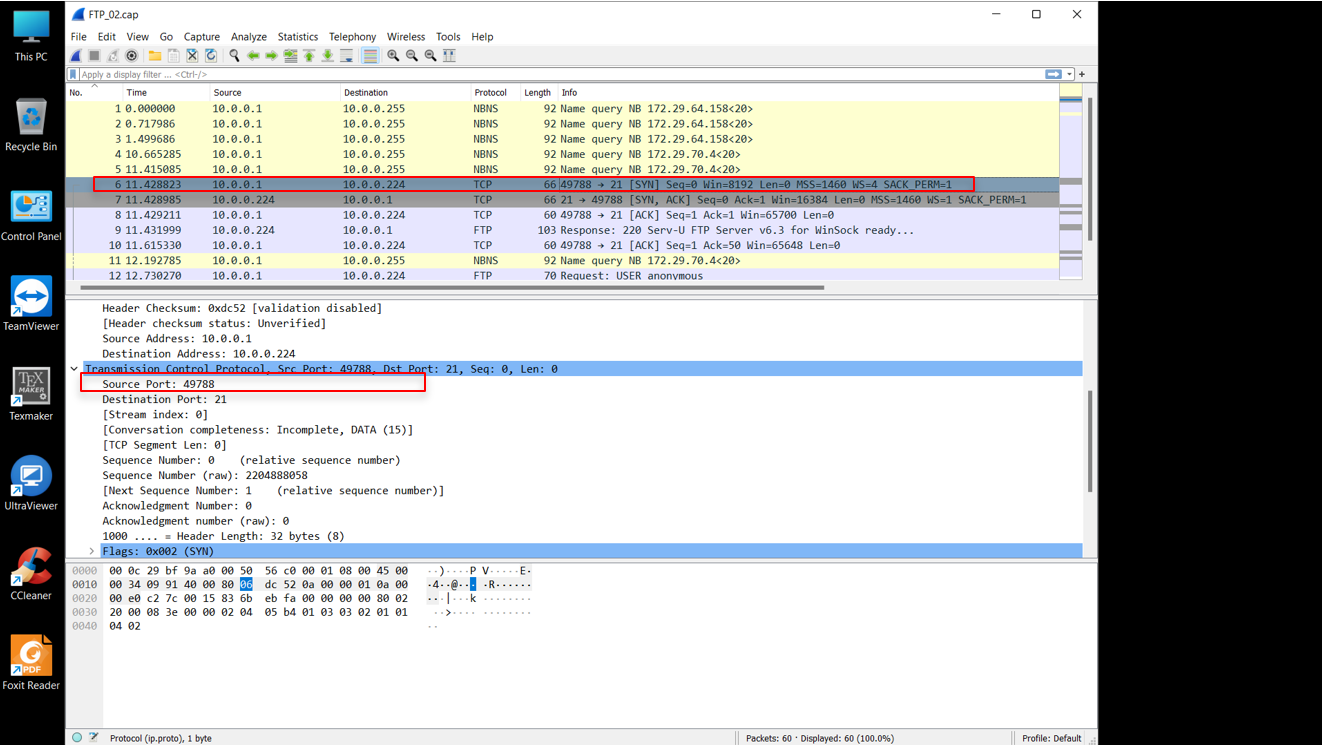
\includegraphics[scale=.8]{../figures/p5/p5_2}
\end{center}
\caption{Port truyền lệnh của client}
%\label{fig5a1}
\end{figure}

\textbf{e.	Client truy xuất lên server theo mode nào: active hay passive?}\\
Client truy xuất lên server theo mode mặc định là active.
Muốn chuyển sang mode passive client cần gửi gói tin request PASV.
\begin{figure}[H]
\begin{center}
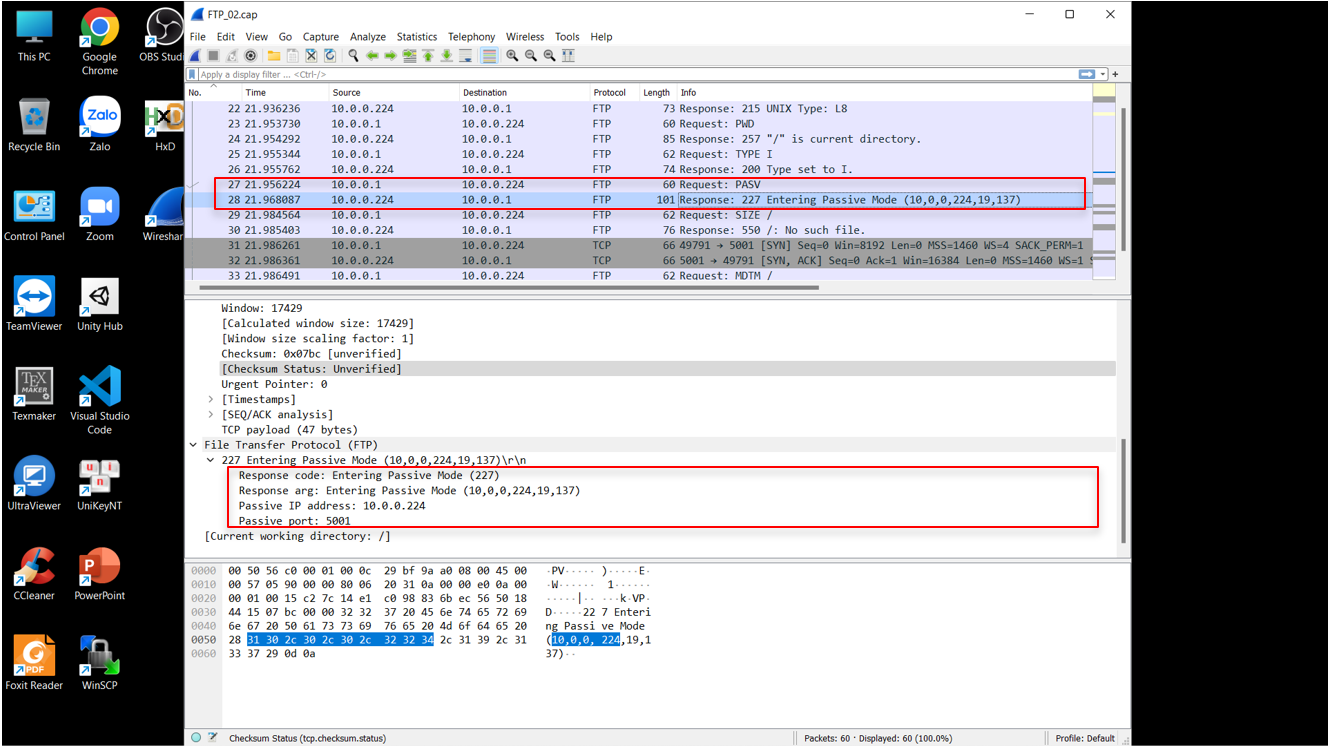
\includegraphics[scale=.8]{../figures/p5/p5_3}
\end{center}
\caption{Thể hiện của gói tin request/response khi muốn vào mode passive}
%\label{fig5a1}
\end{figure}

\textbf{f.	Chỉ ra quá trình bắt tay 3 bước của client và server để tạo kết nối ban đầu khi thực hiện truyền username và password.}
\begin{figure}[H]
\begin{center}
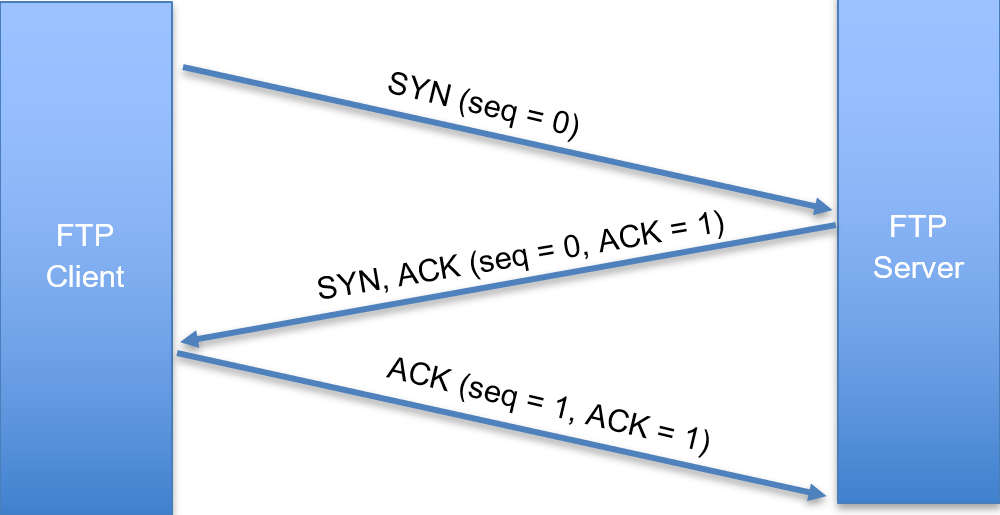
\includegraphics[scale=.6]{../figures/p5/p5_4}
\end{center}
\caption{Quá trình bắt tay 3 bước để tạo kết nối ban đầu}
\end{figure}

\begin{figure}[H]
\begin{center}
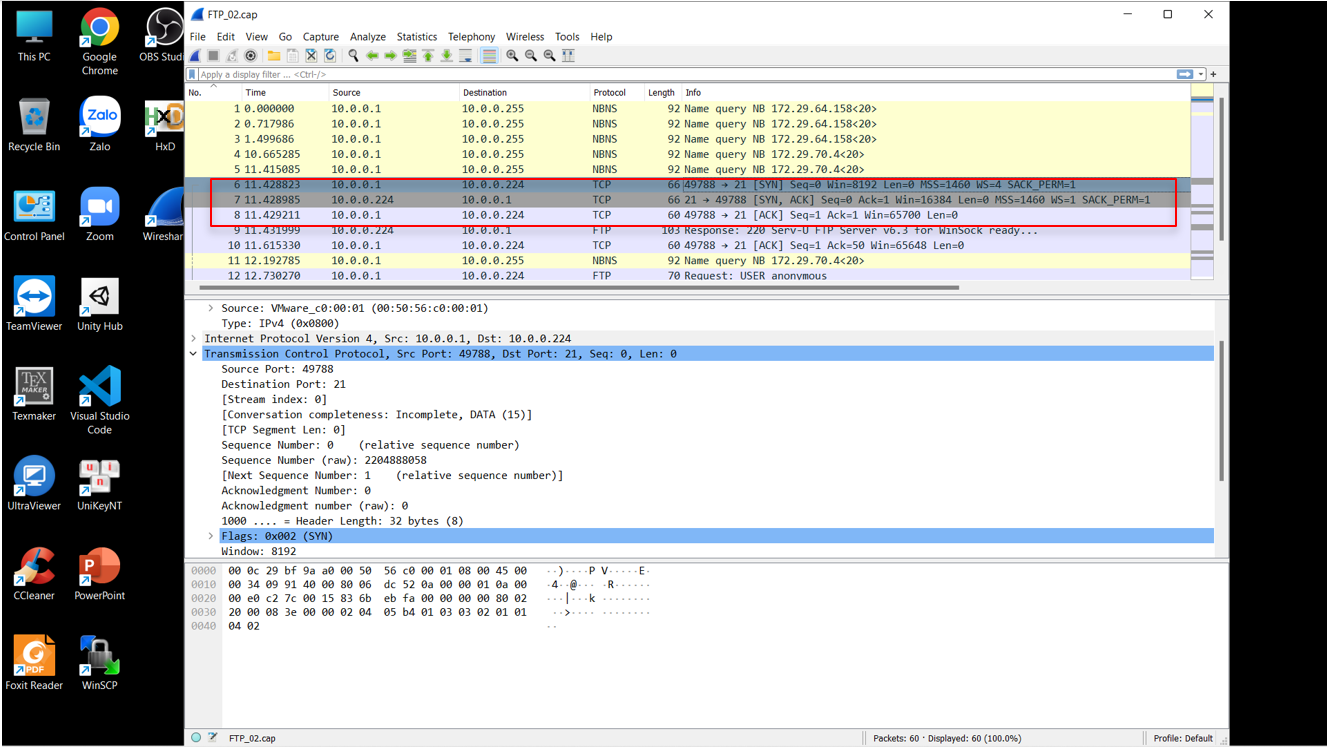
\includegraphics[scale=.8]{../figures/p5/p5_5}
\end{center}
\caption{Quá trình bắt tay 3 bước để tạo kết nối ban đầu}
\end{figure}

\textbf{g.	Chỉ ra quá trình bắt tay 3 bước của client và server để tạo kết nối truyền dữ liệu.}
\begin{figure}[H]
\begin{center}
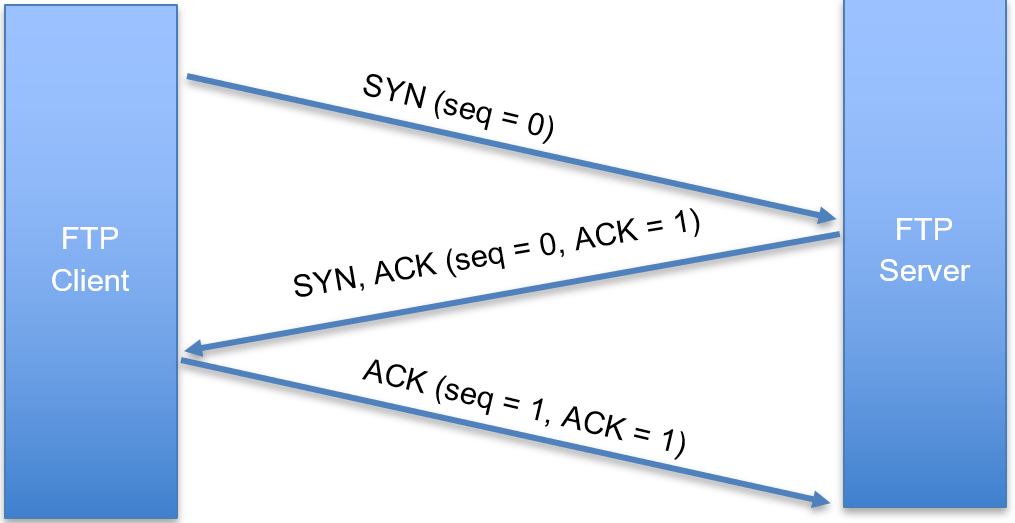
\includegraphics[scale=.6]{../figures/p5/p5_6}
\end{center}
\caption{Quá trình bắt tay 3 bước để tạo kết nối truyền dữ liệu}
\end{figure}

\begin{figure}[H]
\begin{center}
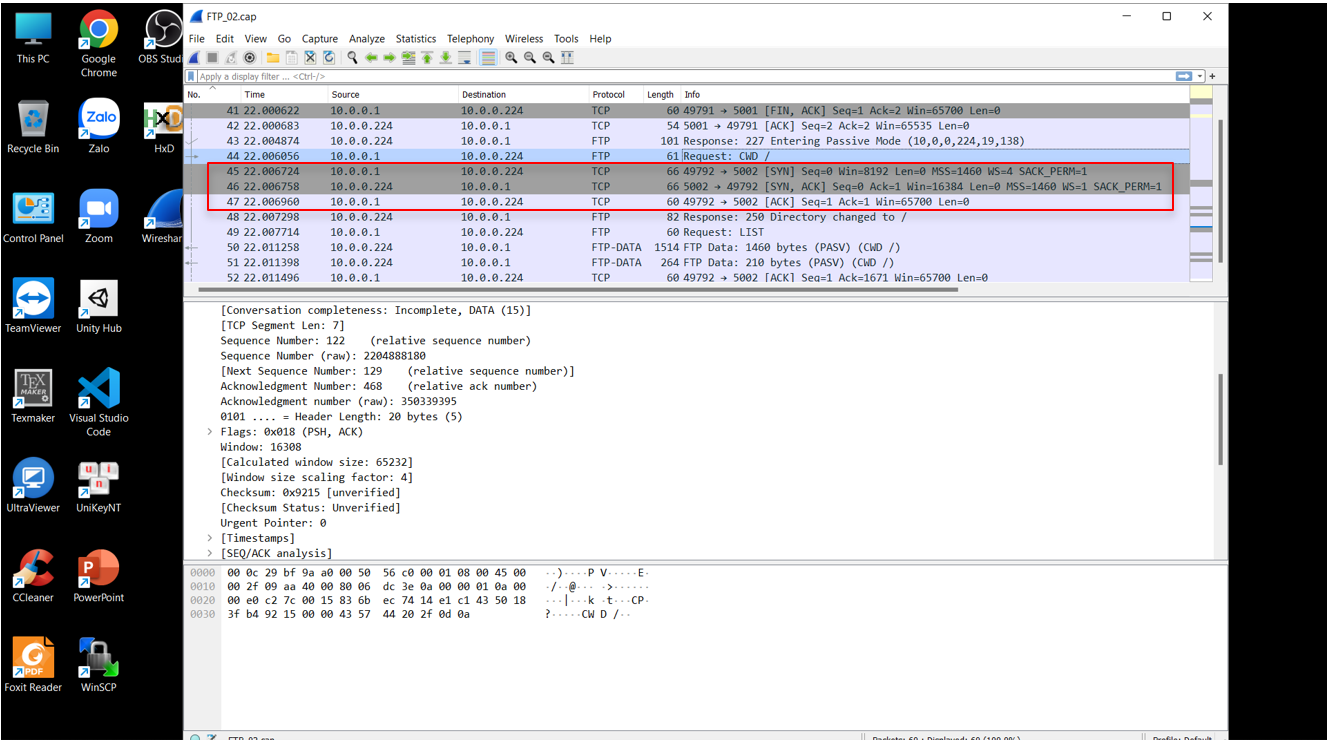
\includegraphics[scale=.8]{../figures/p5/p5_7}
\end{center}
\caption{Quá trình bắt tay 3 bước để tạo kết nối truyền dữ liệu}
\end{figure}

\textbf{h.	Port truyền dữ liệu của FTP server và client là bao nhiêu?}\\
Port truyền dữ liệu của FTP server và client tương ứng là 5002 và 49792. Kết nối này được tạo bởi quá trình bắt tay ba bước ở câu g nêu trên, cụ thể thể hiện ở các gói tin số 45, 46, 47.
Các gói tin liên quan được kẻ khung màu đỏ ở phía trên, khung màu đỏ ở hình \ref{fig5h} (ứng với gói tin số 50, chuyển data từ FTP server sang FTP client) cũng nêu ra port tương ứng.

\begin{figure}[H]
\begin{center}
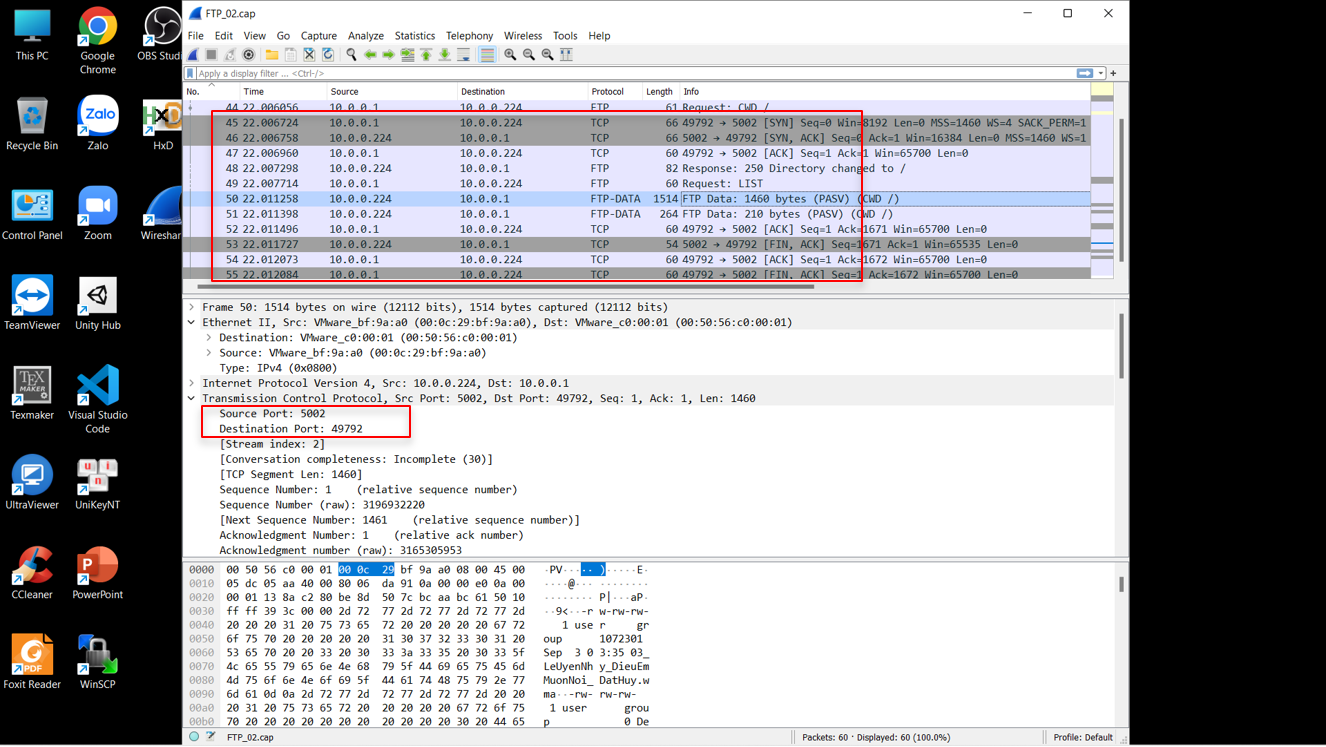
\includegraphics[scale=.8]{../figures/p5/p5_8}
\end{center}
\caption{Port truyền dữ liệu của FTP server và client}
\label{fig5h}
\end{figure}

Trước đó, port truyền dữ liệu của FTP Server và Client tương ứng là 5001 và 49791 (thông tin tương ứng ở các gói tin 31, 32, 34 thể hiện quá trình bắt tay ba bước được nêu ở câu g), và bị ngắt kết nối (các gói tin [FIN,ACK] và [ACK] từ 39 – 42 thể hiện quá trình này).

\nocite{gt}

\newpage
\printbibliography[title = Tài liệu tham khảo]
\end{document}